\documentclass[letterpaper,twoside,12pt]{article}
\usepackage[T1]{fontenc}
\usepackage{textcomp}
%\usepackage[dvips]{graphicx}
\usepackage{graphicx}
\usepackage{epstopdf}
\usepackage[margin=0.8in]{geometry}
\usepackage{caption}
\usepackage{amsmath}
\usepackage{amssymb}
\usepackage[T1]{fontenc}
\usepackage{natbib}
\usepackage{authblk}
%\usepackage{fancyvrb}
%\usepackage{lmodern}
%\usepackage{url}
%\usepackage{times}
\usepackage{textcomp}
%\usepackage{parskip}
\bibliographystyle{agu08}

\newcommand{\ud}{\mathrm d}
\newcommand{\uj}{\mathrm{j}}
\newcommand{\bz}{\mathbf{z}}
\newcommand{\Real}{\mathrm{Re}}
\newcommand{\Imag}{\mathrm{Im}}
\newcommand{\dif}{\mathrm{d}}
\newcommand{\sigsig}{\sigma_1\sigma_2}
\newcommand{\varss}{\varsigma_1\varsigma_2}
\newcommand{\hvarss}{\hat{\varsigma}_1 \hat{\varsigma}_2}
\newcommand{\twodots}{\mathinner {\ldotp \ldotp}}
\newcommand{\midtilde}{\raisebox{0.5ex}{\texttildelow}}

\DeclareMathOperator\erf{erf}

\title{VLBI Session VO2187: Comparison of Pseudo-I Products Before and After Polarization Conversion}

\author[1]{L. V. Benkevitch}
\affil[1]{\small MIT Haystack observatory, Westford, MA 01886, USA.}


\begin{document}

\maketitle

\begin{abstract}

The VGOS data are collected with the use of linearly polarized receivers. However, circular polarization has a number of benefits. The PolConvert software allows VGOS data conversion from linear to circular polarization. In this study we do a statistical comparison of the pseudo-Stokes data before and after the conversion in order to characterize the changes PolConvert introduces.

\end{abstract}


\tableofcontents

\section{VGOS Data}

This study is based on the data acquired during the VLBI session started on 2022-07-06, 18:00 and ended on 2022-07-07, 18:00 with the antennas of the eigth stations listed in Tab.~\ref{stations}.

\begin{table}[ht!]
  \begin{center}
    \caption{Stations in the Schedule for the Session VO2187}
    \label{stations}
    \begin{tabular}{l|l|l|l}
    \multicolumn{2}{c|}{Code} & \multicolumn{1}{c|}{Name} & \multicolumn{1}{c}{Description} \\                       %\multicolumn{2}{c}{Other Headers} \\
     1-ltr & 2-ltr &  &  \\
      \hline
E & Wf & WESTFORD  & Westford, MA, USA \\
G & Gs & GGAO12M  1 &	Goddard Geophysical and Astronomical Observatory (GGAO) \\
H & K2 & KOKEE12M  & Kokee Park Geophysical Observatory \\
I & Is & ISHIOKA   & Ishioka VLBI Station \\
M & Mg & MACGO12M  & McDonald Geodetic Observatory (MGO), TX, USA \\
S & Oe & ONSA13NE  & Onsala 13‐m antenna north‐east, Sweden \\
T & Ow & ONSA13SW  & Onsala 13‐m antenna south‐west, Sweden \\
%V & Ws & WETTZ13S  & Wettzell 13‐m antenna south, Germany \\
Y & Yj & RAEGYEB   & 13‐m at Yebes, Spain
    \end{tabular}
  \end{center}
\end{table}
  


\section{Parameter Temporal Variations Before and After PolConvert}

Converting linear polarization of the source data to the circular polarization with the PolConvert software introduces changes into its parameters. Here we consider the changes in multi-band delays (MBD), single-band delays (SBD), and signal-to-noise ratios (SNR) for the Stokes polarization products, of which we only select the pseudo-Stokes $I$ parameters as functions of time, $t$. The the original VO2107 data set in SWIN (DiFX) format obtained from the stations with linearly polarized antennae is converted into two data sets in the fringe-fit Mark4 format: with linear and circular polarizations. The linearly polarized Mark4 fringe-fit data set is resulted from \verb@difx2mark4@ followed by \verb@fourfit@ conversions. The circularly polarized Mark4 fringe-fit data set requires additional step. First, the PolConvert software converts the original linearly polarized SWIN (DiFX) data set into the circularly polarized SWIN (DiFX) data set. Then the same toolchain of \verb@difx2mark4@ and \verb@fourfit@ converts it into the circularly polarized Mark4 fringe-fit data set. From each of the two data sets we read pseudo-Stokes $I$ of MBD, SBD, and SNR. Below, working with each of these parameters, for $I$ in the two different polarizations we use the names LinI($t$) and CirI($t$). The data are presented in the discrete, numerical format, so instead of the continuous time, $t$, integer indices are used, like $k=\overline{1..N}$, where $N$ is the number of data points in the sample. The following Figures show temporal variations of the LinI[$k$] and CirI[$k$] parameters during the experiment before and after PolConvert, one graph for each baseline:  \\


\indent MBD variations in Fig.~\ref{mbd_lin_and_cir};  \\
\indent SBD variations in Fig.~\ref{sbd_lin_and_cir};  \\
\indent SNR variations in Fig.~\ref{snr_lin_and_cir}.  \\


One can see that most of the graphs after PolConvert, CirI[$k$], are significantly biased with respect to LinI[$k$]. The biases calculated as $\mathrm{LinI}[k] - \mathrm{CirI}[k]$ are plotted in the Figures below: \\

\indent MBD bias variations in Fig.~\ref{mbd_lin_cir_bias};  \\
\indent SBD bias variations in Fig.~\ref{sbd_lin_cir_bias};  \\
\indent SNR bias variations in Fig.~\ref{snr_lin_cir_bias}.  \\

For each of the biases the bias mean, $\overline{\rm Bias}$, is computed.

However, removing the bias by subtracting the mean values of each curve makes the differences much less significant:

\begin{equation}
  \label{subtr_mean_lin}
  \mathrm{LinI}[k] = \mathrm{LinI}[k] - \mathrm{mean(LinI}[k])
\end{equation}

\begin{equation}
  \label{subtr_mean_cir}
  \mathrm{CirI}[k] = \mathrm{CirI}[k] - \mathrm{mean(CirI}[k])
\end{equation}

\noindent In order to compare the unbiased LinI[$k$] with CirI[$k$], the residual, res[$k$], is computed as their difference:

\begin{equation}
  \label{resid}
  \mathrm{res}[k] = \mathrm{LinI}[k] - \mathrm{CirI}[k] 
\end{equation}

\noindent The graphs of residuals with the means subtracted are shown in the following Figures: \\

\indent MBD residual variations in Fig.~\ref{mbd_lin_minus_cir};  \\
\indent SBD residual variations in Fig.~\ref{sbd_lin_minus_cir};  \\
\indent SNR residual variations in Fig.~\ref{snr_lin_minus_cir}.  \\

To assess the similarity of LinI[$k$] and CirI[$k$], the following parameters are computed: \\

\noindent - Pearson correlation coefficient $r_{corr}$; \\
\noindent - Root Mean Square Error, RMSE; \\

Since LinI[$k$] and CirI[$k$] already have their means subtracted, the correlation formula is simplified:

\begin{equation}
  \label{corr}
  r_{corr} = \frac{\sum \mathrm{LinI}[k] \cdot \mathrm{CirI}[k]}{\sqrt{\sum \mathrm{LinI}[k]^2 \cdot 
                   \mathrm{CirI}[k]^2}}
\end{equation}

One can see for most of the baselines the coefficient of the correlation between LinI and CirI shows high values around 0.9 and above.

The root mean square error, RMSE, in our case is actually the standard deviation of the residual, $\sigma$:

\begin{equation}
  \label{rmse}
  \mathrm{RMSE} = \sigma = \sqrt{\frac{1}{N} \sum \mathrm{res}[k]^2}
\end{equation}

Lower RMSE indicates a better fit between the curves. However, RMSE is not an ``absolute'' indicator of the curves' proximity. It needs to be related to the absolute values of both $\mathrm{LinI}$ and $\mathrm{CirI}$. They are shifted, however, to very roughly juxtapose RMSE with the absolute values of the MBD, SBD, and SNR parameters (here denoted as PRM) we have introduced their ``absolute averages'':

\begin{equation}
  \label{abs_avg}
  \overline{\mathrm{PRM}} = \left( \rm |mean(LinI)| + |mean(CirI)| \right)/2.
\end{equation}

To compare the observed values of the parameters LinI and CirI with their unbiased residual RMS error, we write it in the table format with the columns including the time-averaged signal-to-noise ratio $\overline{\rm{SNR}}$, $\overline{\mathrm{PRM}} \pm \mathrm{RMSE}$ or $\overline{\mathrm{PRM}} \pm \sigma$, the relative error (\%), the time-averaged bias between LinI and CirI, $\overline{\rm{Bias}}\, (ps)$, and the correlation coefficient, $r_{corr}$, for each of the baselines. The relative error between the unbiased LinI and CirI can be expressed as

\begin{equation}
  \label{rel_err}
  \rm relerr (\%) = RMSE / \overline{\mathrm{PRM}}.
\end{equation}

These characteristics are summarized in the Tables Appendix: \\

\noindent MBD PolConversion parameters in Table~\ref{mbd_conv_param}; \\
\noindent SBD PolConversion parameters in Table~\ref{sbd_conv_param}; \\
\noindent SNR PolConversion parameters in Table~\ref{snr_conv_param}. \\



\section{Parameter residual Statistics Before and After PolConvert}

In the previous Section MBD, SBD, and SNR pseudo-Stokes $I$ parameter data were shown as functions of time. Here we conduct their statistical study. In order to estimate the errors introduced by PolConvert, histograms of the unbiased parameter residuals (after the mean subtraction, see Eqs.~\eqref{subtr_mean_lin} and \eqref{subtr_mean_cir}) are plotted. Below are the histograms for all of the baselines: \\

\indent MBD residual histogram for all of the baselines in Fig.~\ref{dmbd_distr};  \\
\indent SBD residual histogram for all of the baselines in Fig.~\ref{dsbd_distr};  \\
\indent SNR residual histogram for all of the baselines in Fig.~\ref{dsnr_distr}.  \\

It is interesting to see which of the individual stations contribute to the errors. We plotted histograms of the parameter residuals for the baselines involving each particular station. They are shown in the following Figures: \\

\indent MBD residual histograms for the baselines including one station in Fig.~\ref{dmbd_distr_st};  \\
\indent SBD residual histograms for the baselines including one station in Fig.~\ref{dsbd_distr_st};  \\
\indent SNR residual histograms for the baselines including one station in Fig.~\ref{dsnr_distr_st}.  \\

In order to evaluate the significance of the error we attempted to use the Pearson's chi-squared test comparing the histograms to the normal distributions:

\begin{equation}
  \label{normal_pdf}
  f(\mu,\sigma) =  \frac{1}{\sigma\sqrt{2\pi}} e^{-\frac{(x-\mu)^2}{2\sigma^2}}.
\end{equation}

All the histograms of residuals are computed for 41 bins. However, the histograms have long tails filled with zeros or small numbers because the data have occasional outlier points far from their means. Plotting such distributions with all the bins makes the histohrams too narrow and their most significant portions near the means are poorly visible. Therefore, to plot them and to perform the Pearson's $\chi^2$ test, the left-tail and right-tail bins with sparse data (frequencies less than 8) were grouped and the test used fewer number of bins $N_b$ (see it printed in each plot, Fig.~\ref{dmbd_distr} - Fig. \ref{dsnr_distr_st}). The Pearson's $\chi^2$ test compares the observed data counts in the bins $B_i$ with the expected (theoretical) counts $E_i$, where $i=\overline{1 \twodots N_b}$, obtained from the normal PDF~\eqref{normal_pdf} as $E_i = Np_i$. Here $p_i$ is the probability that a random value sampled from $f(\mu,\sigma)$ is within the $i$-th interval. The value of the test-statistic is calculated as
\begin{equation}
  \label{x2_calc}
  X^2 = \sum_{i=1}^{N_b} \frac{(B_i - E_i)^2}{E_i},
\end{equation}
where $N_b$ is the number of bins.
The $X^2$ test statistic asymptotically approaches the $\chi^2_\mathrm{df}$ distribution, where $\mathrm{df}$ is the number of degrees of freedom:
\begin{equation}
  \label{df}
  \mathrm{df} = N_b - k - 1,
\end{equation}
where $k=2$ is the number of parameters estimated from the data, mean $\mu$ and standard deviation $\sigma$. The additional $-1$ is due to the fact that the $\chi^2$ test itself has a restriction imposed by the sum of the observed frequencies being equal to the sum of the expected frequencies.

If we want to be 95\% confident that the data is distributed normally, $X^2$ cannot exceed the critical value $\chi^2_{cr}$ such that the probability for $X^2$ to appear within the interval $[0 \twodots \chi^2_{cr}]$ is $p=0.95$. Hence we should set the level of significance $\alpha = 1 - p = 0.05$.  The critical $\chi^2_\mathrm{df}$ value can be calculated as the value of $\chi^2$ Probability Point Function (PPF), the inverse of the $\chi^2$ Cumulative Distribution Function or CDF. In Python this is done as $\verb@scipy.stats.chi2.ppf(1-alpha, df)@$. Alternatively, the Inverse Survival Function (ISF) may be used as $\verb@scipy.stats.chi2.isf(alpha, df)@$.

Unfortunately, in our case the Pearson's $\chi^2$ test fails, because the residuals are grouped around their means substantially denser than the normal distributions with the same standard deviations. In most distributions, the calculated values of the histogram chi-squares are many times greater than the critical chi-square values for the p-values less than or equal to 0.05 (printed in each of the histogram plots).
So, we had to use another method to assess how close are the parameter values before (LinI[i]) and after (CirI[i]) the polarization conversion. Since most of the residuals LinI[i] - CirI[i] are within $\pm \sigma$ (standard deviation), we  compute their proportion and compare it to the expected proportion under a normal distribution, which is about 68.27\%. The proportion is printed near each histogram. It is at the level of about 80\%-90\% and more, which is better than the standard normal distribution for all the histograms considered.




\section{Conclusion}

We have conducted a study to assess how well the PolConvert software makes VGOS data conversion from linear to circular polarization. The pseudo-Stokes data of the Multi-Band Delays (MBD), Single-Band Delays (SBD), and Signal-to-Noise Ratios (SNR) as functions of time before and after the conversion were plotted as functions of time for visual inspection. We also did a statistical comparison of the pseudo-Stokes data of MBD, SBD, and SNR before and after the conversion in order to characterize the variations PolConvert introduces. Two criteria were used to assess the residuals: the Pearson's $\chi^2$ test and the proportions of residuals within $\pm\sigma$ compared to the normal distribution. 

PolConvert introduces large (and random) biases between the pseudo-Stokes data parameters. 

On the other hand side, after the bias removal, the average errors (computed as unbiased rms residual) are very small making tenths of percent for the most of baselines for MBD (see Table~\ref{mbd_conv_param}) and SNR (see Table~\ref{snr_conv_param}). For SBD the relative error is an order of magnitude greater. The SBD conversion biases are generally larger, too (see Table~\ref{sbd_conv_param}).

The unbiased residuals generally have good distributions, denser than the normal with the same STD, as can be seen in Figs.~\ref{dmbd_distr} to~\ref{dsnr_distr_st}.

\cleardoublepage

\section{Appendix: Software}

\subsection{make\_sorted\_idx\_2187.py: Saving VGOS data in Python dictionaries}

The VLBI Global Observing System (VGOS) database is organized as a directory structure. For our purpose of statistical analysis of a small number of parameters scattered across many directories and files below the root directory of the experiment, this implies significant overhead in opening multiple files and accessing the parameters in each of them. The data files in their names only provide the station or baseline names, and no time or polarization information. For example, extraction of, say, SNR data for a particular polarization product and within a specific time range would require opening \emph{all} the files and accessing their times and polarizations using HOPS API calls.

I wrote a script, \verb@make_sorted_idx_2187.py@, to extract the parameters for statistical analysis for the whole experiment and to put it in a Python dictionary, preserving the temporal order. I call such dictionaries ``indices''. The index can be ``pickled'' and saved on disk. These files are small, in the hundreds of kilobytes to one-two megabytes.  The scripts for data analisys and plotting read the index files, unpickle them into the Python dictionaries, and use data from the dictionaries.

A pickle file can be unpickled into a  dictionary using the \verb@pickle.load()@ function. For example: \\ \\
\noindent \verb@import pickle@ \\
\noindent \verb@with open('idx2187cI.pkl', 'rb') as finp:@ \\
\noindent \verb@    idx2187c = pickle.load(finp)@ \\ \\

\noindent The script \verb@make_sorted_idx_2187.py@ is also a Python module defining the function \\ \\
\verb@make_idx(base_dir, pol='lin', max_depth=2)@ with parameters: \\ \\
\verb@    base_dir@: the directory containing the VGOS data. For example, it may be \\
\verb@              Work/2187/@. \\
\verb@    pol@: polarization, 'lin' - linear, 'cir' - circular. \\
    \indent \indent \indent This parameter is used for the data generated by PolConvert. \\
    \indent \indent \indent It converts the polarization product names\\
    \verb@          'XX', 'XY', 'YX', 'YY'@, and the lists \verb@['XX', 'YY']@ into the correct names \\
    \verb@          'LL', 'LR', 'RL', 'RR'@, and \verb@'I'@, respectively. \\
\verb@    max_depth@: Limits the maximum depth of recursing into the subdirectories of \verb@base_dir@. \\

\noindent \verb@make_idx()@ creates and returns the index dictionary with the data from \verb@base_dir@. \\

The index dictionary has three dimensions: the baseline name, the polarization, and the data proper, including 'time', 'file', 'mbdelay', 'sbdelay', and 'snr'. Consider a particular index named \verb@idx2187l@ (experiment 2187, linear polarization). Its first dimension is indexed with the baseline names derived from the set of stations, \verb@{'E', 'M', 'S', 'T', 'V', 'Y'}@. \\
\noindent The possible first indices are the baseline names: \\
\verb@idx2187l.keys()@ \\
\verb@dict_keys(['SE', 'VY', 'MV', 'MT', 'TV', 'EY', 'SY', 'TY', 'MS', 'SV',@ \\
\verb@           'TE', 'EV', 'MY', 'ME'])@ \\ \\
\noindent Each of the baselines is associated with the cross-corellation products and the pseudo-Stokes I parameter. Thus the second index is one of the products. For example, for the \verb@'ME'@ baseline: \\
\verb@idx2187l['ME'].keys()@ \\
\verb@dict_keys(['XX', 'XY', 'YX', 'YY', 'I'])@ \\ \\
For example, the times, the full data file names, SNRs, multi- and single-band delays for the 'SY' baseline and the 'XY' polarization products from this baseline are contained in the index dictionary under \\
\verb@idx2187l['SY']['XY']@: \\ \\
\verb@idx2187l['SY']['XY'].keys()@ prints \\
\verb@dict_keys(['time', 'file', 'mbdelay', 'sbdelay', 'snr'])@. \\ \\
For example, in order to access the multi-band delay data list in the ascending temporal order for the baseline \verb@'SV'@ and the pseudo-Stokes I, one should issue the following command: \\
\verb@mbd = idx2187l['SV']['I']['mbdelay'].@

\subsection{group\_tails.py: Group Tail Bins with Sparse Data}

\verb@group_tails.py@ is a Python module defining the functions \verb@find_tail_bounds(ni, fni)@ and \verb@group_tails(ni [, thr=5])@: \\

Usage: \\
\verb@from group_tails import find_tail_bounds, group_tails@ \\
\verb@l_idx, r_idx = find_tail_bounds(ni)@ \\
\verb@ni =  group_tails(ni,  (l_idx, r_idx)) @ \\

\noindent \verb@find_tail_bounds(ni)@: \\
- finds two indices, left and right, at which the sparse tails of \verb@ni@ to be cut after grouping. The tail is considered sparse if it contains values less than ot equal the threshold \verb@thr@. 

The input parameter of \verb@find_tail_bounds(ni)@ is an array containing a distribution of observed frequencies. The \verb@find_tail_bounds(ni)@ function outputs the indices, \verb@(l_idx, r_idx)@, where \\
\verb@    l_idx@ points AT the first ni element greater than thr, and \\
\verb@    r_idx@ points AFTER the last ni element greater than thr.

\noindent So, \verb@ni[l_idx:r_idx]@ is the subarray whose elements are > thr at either ends. \\

\noindent \verb@group_tails(ni,  (l_idx, r_idx))@: \\
- sums up the sparse tail values in \verb@ni@ and adds them to the border values on the either side. \\
\noindent - outputs the array \verb@ni_grp@, the result of the sparse tails grouping of \verb@ni@.

Using the tail indices \verb@(l_idx, r_idx)@ one can make the tail grouping on the same size array \verb@fni@ of expected (theoretical) frequencies, calculated from a distribution to which \verb@ni@ has been fit:
\verb@fni =  group_tails(fni,  (l_idx, r_idx))@.


\subsection{Plot Parameter Temporal Variations}

The script \verb@plot_time_par_2187_2187.py@ creates plots for MBD, SBD, and SNR time variations. The data are read from the dictionaries \verb@idx2187lI.pkl@ and \verb@idx2187cI.pkl@.\\

\noindent Usage: \\
\verb@$ python plot_time_par_2187.py <par> [save], @ \\
\verb@       where <par> is either MBD or SBD or SNR (lower case permitted).@ \\
\verb@       save (optional): save figures in pdf format.@ \\

\noindent The plots generated are shown in Figures~\ref{mbd_lin_and_cir} to~\ref{snr_lin_minus_cir}.



\subsection{Plot Parameter Histograms}

The script \verb@plot_st_difhist_2187.py@ creates histograms of the residual distributions for MBD, SBD, and SNR. The residuals are differences between 
the pseudo-Stokes I parameters before and after the PolConvert. The data are read from the dictionaries \verb@idx2187l.pkl@ and \verb@idx2187cI.pkl@.
\\

\noindent Usage: \\
\verb@$ python plot_st_difhist_2187.py <par> [save], @ \\
\verb@       where <par> is either MBD or SBD or SNR (lower case permitted).@ \\
\verb@       save (optional): save figures in pdf format.@ \\

\noindent The plots generated are shown in Figures~\ref{dmbd_distr} to~\ref{dsnr_distr_st}.


\cleardoublepage

\section{Appendix: Tables}

\begin{table}[ht!]
  \begin{center}
    \caption{Pseudo-Stokes I MBD PolConversion Parameters}
    \label{mbd_conv_param}
    \begin{tabular}{l|r|r|c|r|r}
      BL & $\overline{\rm{SNR}}$ & $\overline{\rm{MBD}}\pm\sigma\, (ps)$ & \text{relerr (\%)} & $\overline{\rm{Bias}}\, (ps)$ & \multicolumn{1}{c}{$r_{corr}$} \\
      \hline
      GE & 102.5 & $3225.3 \pm    2.0$ &   0.06 &  -686.2 & 0.999986 \\
      GH &  91.7 & $4111.4 \pm  674.5$ &  16.40 &  -869.3 & 0.959041 \\
      GI &  53.9 & $2414.4 \pm  916.4$ &  37.96 &  -951.9 & 0.946194 \\
      GM & 104.5 & $ 297.4 \pm  320.7$ & 107.85 &   345.1 & 0.984252 \\
      GS & 104.8 & $ 534.3 \pm  423.6$ &  27.61 &  -225.0 & 0.980334 \\
      GT & 113.0 & $1982.8 \pm  433.7$ &  21.87 & -1189.7 & 0.979027 \\
      HE &  82.2 & $ 710.6 \pm  645.6$ &  90.86 &   198.2 & 0.759337 \\
      HM & 121.9 & $2669.1 \pm  860.4$ &  32.23 &  1129.1 & 0.875116 \\
      HS &  97.1 & $2428.3 \pm  666.3$ &  27.44 &   551.5 & 0.902311 \\
      HT & 103.6 & $1948.1 \pm  698.4$ &  35.85 &  -440.9 & 0.892581 \\
      IE &  54.1 & $ 163.4 \pm  660.3$ & 404.18 &   326.7 & 0.907950 \\
      IH &  79.7 & $ 183.0 \pm 1310.7$ & 716.20 &   295.7 & 0.705438 \\
      IM &  64.1 & $2005.6 \pm 1159.0$ &  57.78 &  1035.4 & 0.885539 \\
      IS &  70.5 & $1486.7 \pm 1474.5$ &  99.18 &   711.1 & 0.667996 \\
      IT &  75.2 & $1076.8 \pm 1271.6$ & 118.10 &  -137.5 & 0.721770 \\
      ME &  94.9 & $2404.2 \pm  386.4$ &  16.07 &  -977.8 & 0.872342 \\
      MS &  98.1 & $ 678.9 \pm  531.6$ &  78.30 &  -436.5 & 0.922517 \\
      MT & 102.8 & $1050.8 \pm  540.8$ &  51.46 & -1402.0 & 0.913555 \\
      SE &  97.4 & $1587.4 \pm  391.0$ &  24.63 &  -481.4 & 0.916335 \\
      TE & 107.9 & $1072.9 \pm  398.0$ &  37.09 &   492.0 & 0.913627 \\
    \end{tabular}
  \end{center}
\end{table}


\begin{table}[ht!]
  \begin{center}
    \caption{Pseudo-Stokes I SBD PolConversion Parameters}
    \label{sbd_conv_param}
    \begin{tabular}{l|r|r|c|r|r}
      BL & $\overline{\rm{SNR}}$ & $\overline{\rm{SBD}}\pm\sigma\, (ps)$ & \text{relerr (\%)} & $\overline{\rm{Bias}}\, (ps)$ & \multicolumn{1}{c}{$r_{corr}$} \\
      \hline
      GE & 102.5 & $ 2978.3 \pm   84.2 $ &    2.83 &   319.1 &  0.956047 \\
      GH &  91.7 & $ 4690.5 \pm  365.2 $ &    7.79 &   902.8 &  0.989360 \\
      GI &  53.9 & $ 2351.5 \pm 4417.6 $ &  187.87 &   909.2 &  0.463318 \\
      GM & 104.5 & $ 1825.1 \pm  215.0 $ &   11.78 &  1497.9 &  0.993014 \\
      GS & 104.8 & $ 2094.7 \pm  259.0 $ &   12.36 &   940.5 &  0.992972 \\
      GT & 113.0 & $ 2157.8 \pm  206.5 $ &    9.57 &   566.3 &  0.995751 \\
      HE &  82.2 & $ 1485.2 \pm  367.7 $ &   24.76 &  -579.3 &  0.967322 \\
      HM & 121.9 & $ 1753.4 \pm  413.7 $ &   23.59 &   592.7 &  0.982415 \\
      HS &  97.1 & $ 2334.3 \pm  273.7 $ &   11.73 &   180.0 &  0.981453 \\
      HT & 103.6 & $ 2176.8 \pm  261.5 $ &   12.01 &   -67.3 &  0.984784 \\
      IE &  54.1 & $  189.2 \pm 3996.7 $ & 2112.57 &  -378.4 &  0.689708 \\
      IH &  79.7 & $  545.2 \pm 8128.4 $ & 1490.91 &  1090.4 &  0.484396 \\
      IM &  64.1 & $  356.9 \pm  600.5 $ &  168.25 &   527.4 &  0.955738 \\
      IS &  70.5 & $ 1006.4 \pm 4542.5 $ &  451.38 &   104.3 &  0.188261 \\
      IT &  75.2 & $ 1004.2 \pm 6604.8 $ &  657.72 &   198.8 & -0.020218 \\
      ME &  94.9 & $  678.5 \pm  236.1 $ &   34.79 & -1171.3 &  0.970733 \\
      MS &  98.1 & $  252.4 \pm  241.6 $ &   95.74 &  -504.8 &  0.988171 \\
      MT & 102.8 & $  380.9 \pm  231.2 $ &   60.69 &  -761.7 &  0.988901 \\
      SE &  97.4 & $  993.0 \pm  249.0 $ &   25.07 &  -673.3 &  0.980868 \\
      TE & 107.9 & $  777.2 \pm  248.6 $ &   31.98 &  -293.0 &  0.983206 \\
    \end{tabular}
  \end{center}
\end{table}

\begin{table}[ht!]
  \begin{center}
    \caption{Pseudo-Stokes I SNR PolConversion Parameters}
    \label{snr_conv_param}
    \begin{tabular}{l|r|c|r|r}
      %BL & \multicolumn{1}{c}{$\overline{\rm{SNR}}\pm\sigma$} & \text{relerr (\%)} & $\overline{\rm{Bias}}$ & & \multicolumn{1}{c}{$r_{corr}$} \\
      BL & \multicolumn{1}{c}{$\overline{\rm{SNR}}\pm\sigma$} & \text{relerr (\%)} & $\overline{\rm{Bias}}$ & \multicolumn{1}{c}{$r_{corr}$} \\
      \hline
      GE & $ 102.5 \pm  1.0 $ &  0.99 &  1.1 & 0.999915 \\
      GH & $  91.7 \pm 12.2 $ & 13.28 &  9.8 & 0.980171 \\
      GI & $  53.9 \pm  6.7 $ & 12.45 &  5.7 & 0.963876 \\
      GM & $ 104.5 \pm  7.7 $ &  7.37 &  7.7 & 0.995619 \\
      GS & $ 104.8 \pm  9.0 $ &  8.63 &  5.4 & 0.988439 \\
      GT & $ 113.0 \pm 10.4 $ &  9.17 &  4.8 & 0.987994 \\
      HE & $  82.2 \pm  8.8 $ & 10.67 &  8.1 & 0.982994 \\
      HM & $ 121.9 \pm 17.8 $ & 14.61 & 17.7 & 0.983780 \\
      HS & $  97.1 \pm 13.4 $ & 13.75 &  9.2 & 0.959090 \\
      HT & $ 103.6 \pm 13.0 $ & 12.59 &  8.2 & 0.965008 \\
      IE & $  54.1 \pm  5.8 $ & 10.76 &  5.1 & 0.965831 \\
      IH & $  79.7 \pm 10.6 $ & 13.35 &  8.3 & 0.984451 \\
      IM & $  64.1 \pm 12.4 $ & 19.35 & 13.2 & 0.959665 \\
      IS & $  70.5 \pm  7.0 $ &  9.94 &  4.1 & 0.984968 \\
      IT & $  75.2 \pm  7.1 $ &  9.47 &  3.6 & 0.987480 \\
      ME & $  94.9 \pm  6.0 $ &  6.31 &  6.9 & 0.995813 \\
      MS & $  98.1 \pm  8.1 $ &  8.21 & 10.2 & 0.990928 \\
      MT & $ 102.8 \pm  8.2 $ &  8.01 & 10.2 & 0.990570 \\
      SE & $  97.4 \pm  7.9 $ &  8.06 &  4.9 & 0.989331 \\
      TE & $ 107.9 \pm  9.3 $ &  8.57 &  5.3 & 0.988900 \\      
    \end{tabular}
  \end{center}
\end{table}




\cleardoublepage

\section{Appendix: Figures}


\begin{figure}[ht!]
  \begin{center}
  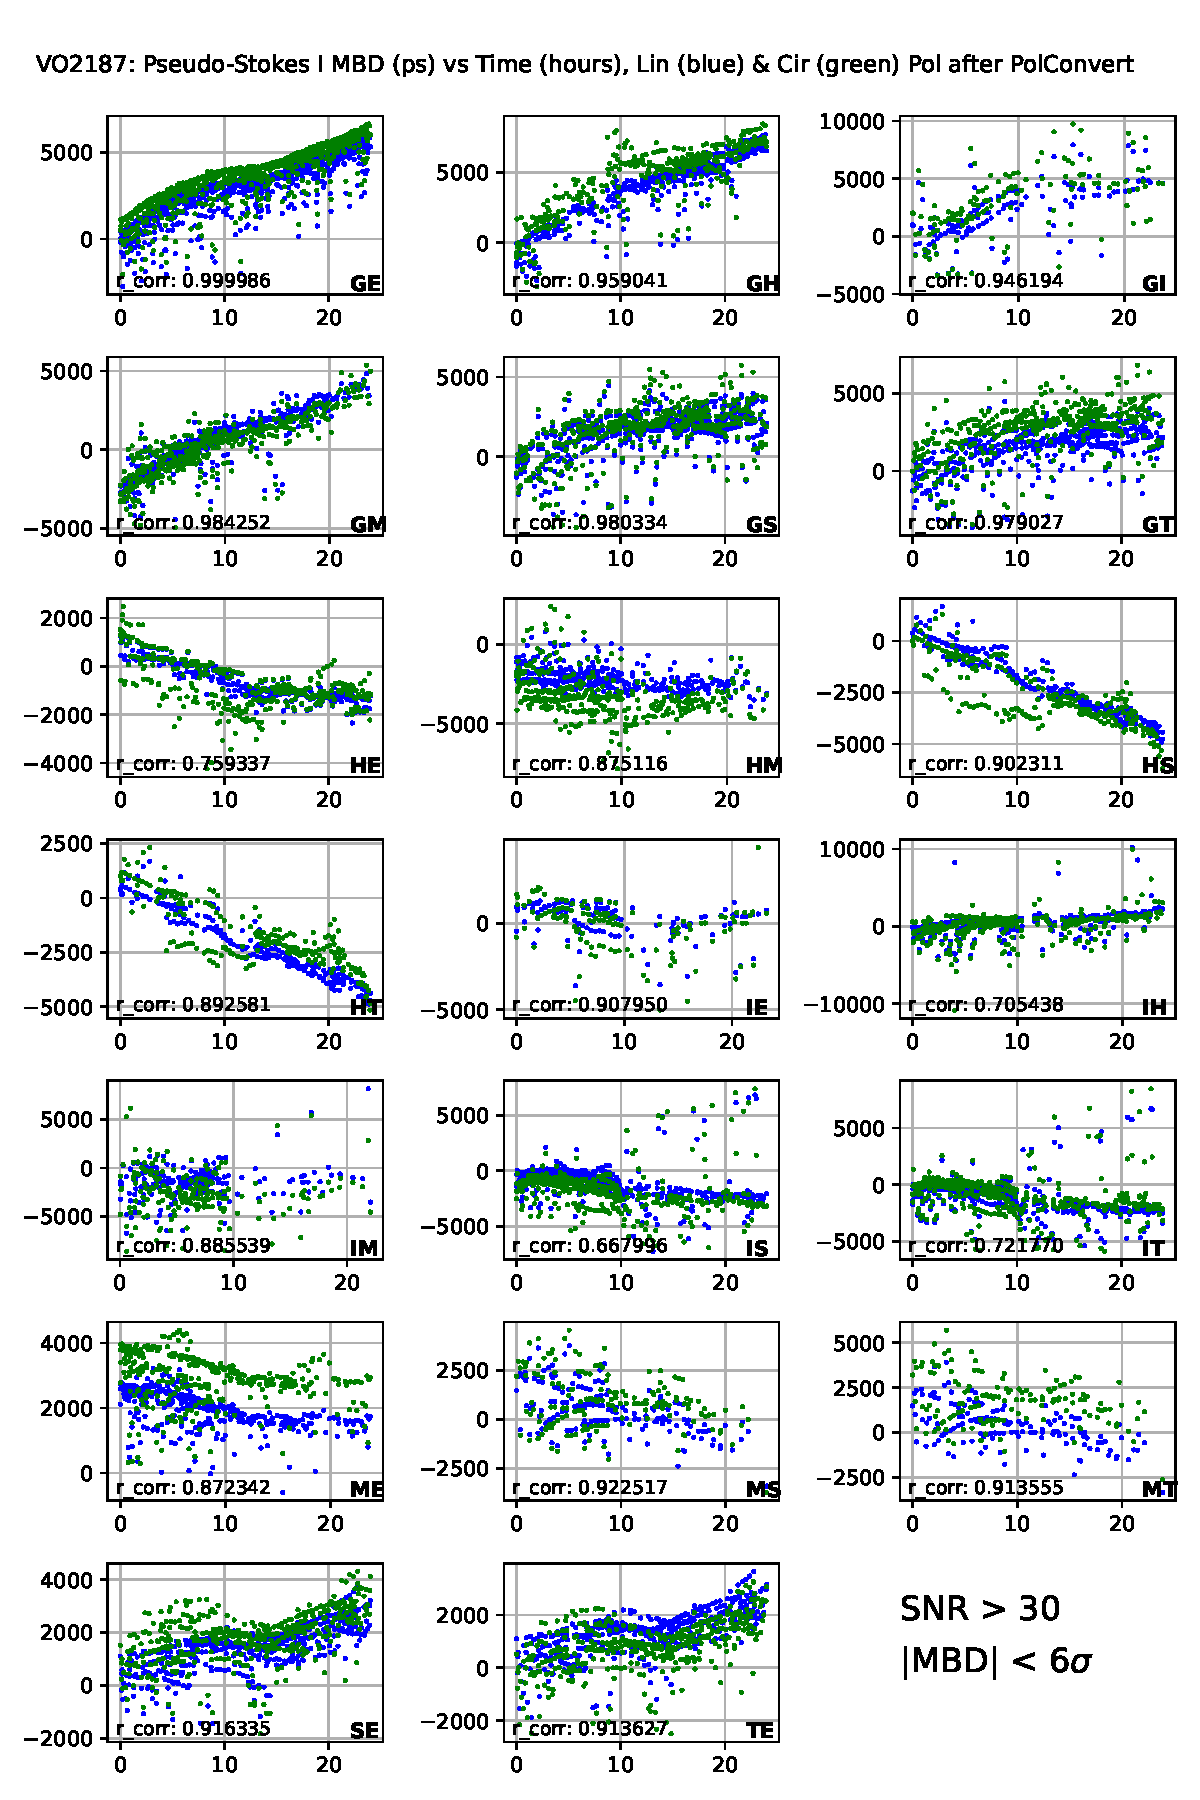
\includegraphics[width=33pc]{VO2187_MBD_Lin_I_and_Cir_I_SNR_floor_30.pdf}
  \caption{\small Evolution of Multi-Band Delays (in picoseconds) during the experiment (time in minutes) for the pseudo-Stokes $\protect I$ parameter for every baseline. Each panel shows two curves: LinI, $\protect I$ from the original, linearly polarized data set and CirI, $\protect I$ from the circularly polarized data set obtained by applying PolConvert to the original data. Graphs have large biases. However, the coefficients of correlation r\_corr between LinI and CirI are very close to unity.}
  \label{mbd_lin_and_cir}
  \end{center}
\end{figure}


\begin{figure}[ht!]
  \begin{center}
  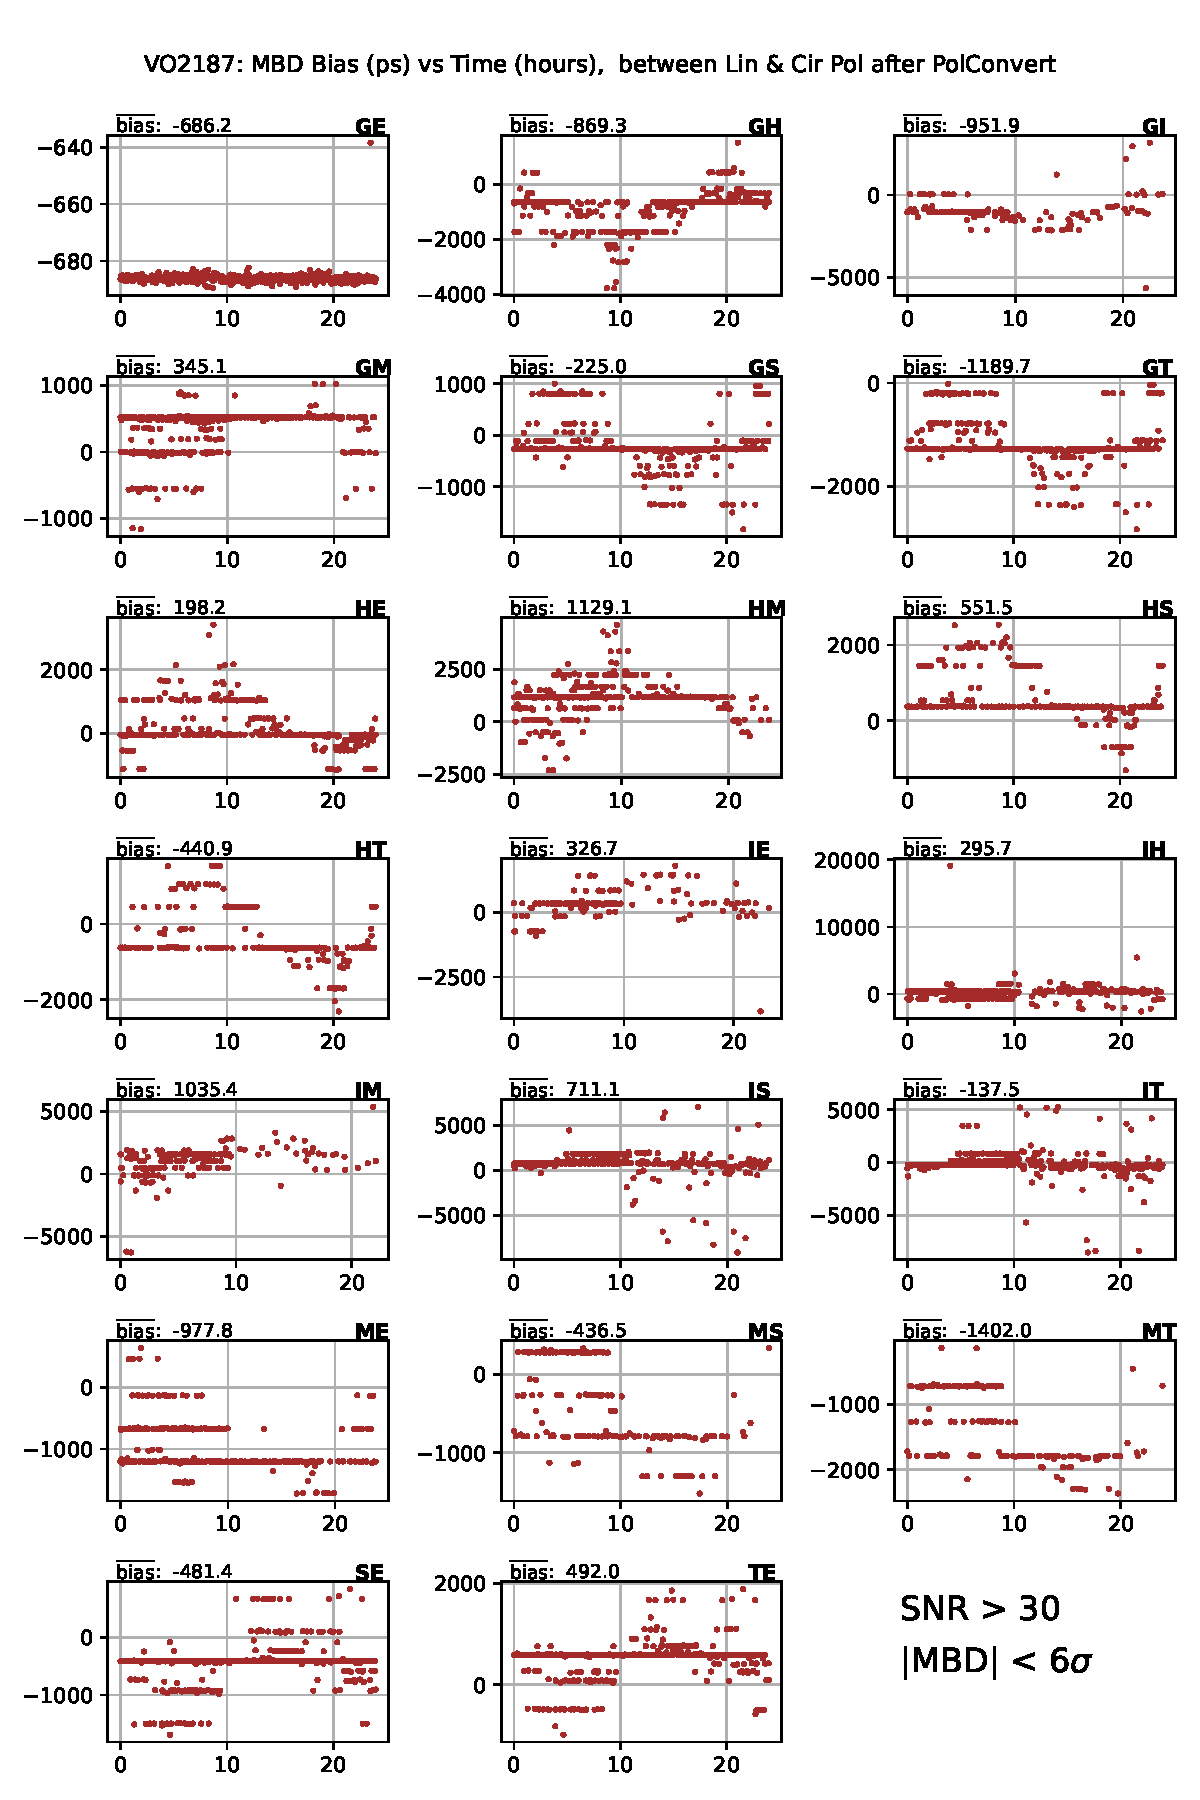
\includegraphics[width=33pc]{VO2187_MBD_bias_between_Lin_I_and_Cir_I_SNR_floor_30.pdf}
  \caption{\small Evolution of the bias between LinI and CirI Multi-Band Delays (in picoseconds) during the experiment (time in minutes) for the pseudo-Stokes $\protect I$ parameter for every baseline. Each panel shows one curve of LinI - CirI, where LinI is $\protect I$ from the original, linearly polarized data set and CirI is $\protect I$ from the circularly polarized data set obtained by applying PolConvert to the original data. The means for each curve are given.}
  \label{mbd_lin_cir_bias}
  \end{center}
\end{figure}


\begin{figure}[ht!]
  \begin{center}
  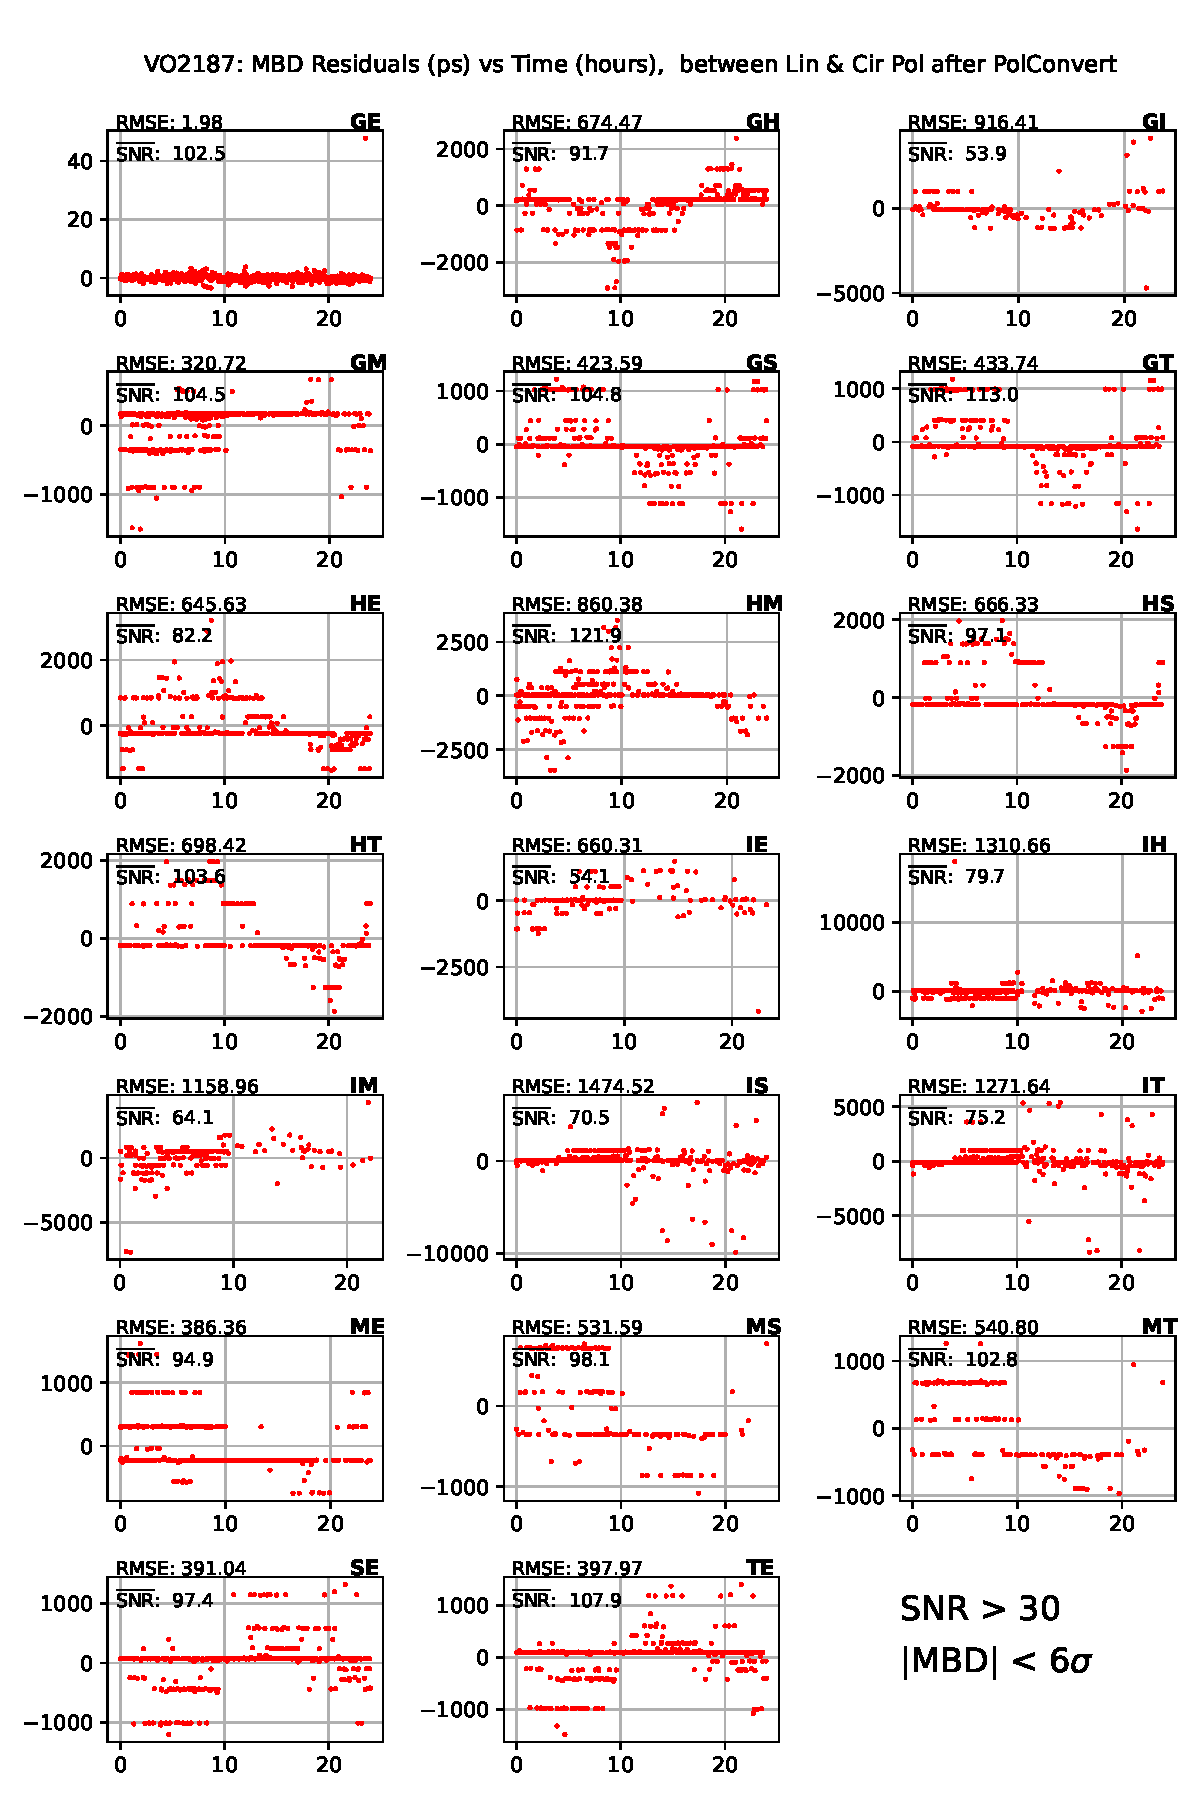
\includegraphics[width=33pc]{VO2187_MBD_Lin_I_minus_Cir_I_SNR_floor_30.pdf}
  \caption{\small Evolution of the residuals between unbiased LinI and CirI Multi-Band Delays (in picoseconds) during the experiment (time in minutes) for the pseudo-Stokes $\protect I$ parameter for every baseline. Each panel shows a curve of LinI - CirI, both with subtracted means, where LinI is $\protect I$ from the original, linearly polarized data set and CirI is $\protect I$ from the circularly polarized data set obtained by applying PolConvert to the original data. The time-averaged SNRs are given. The Root Mean Square Error (RMSE) shows the standard deviation of the residuals.}
  \label{mbd_lin_minus_cir}
  \end{center}
\end{figure}


\begin{figure}[ht!]
  \begin{center}
  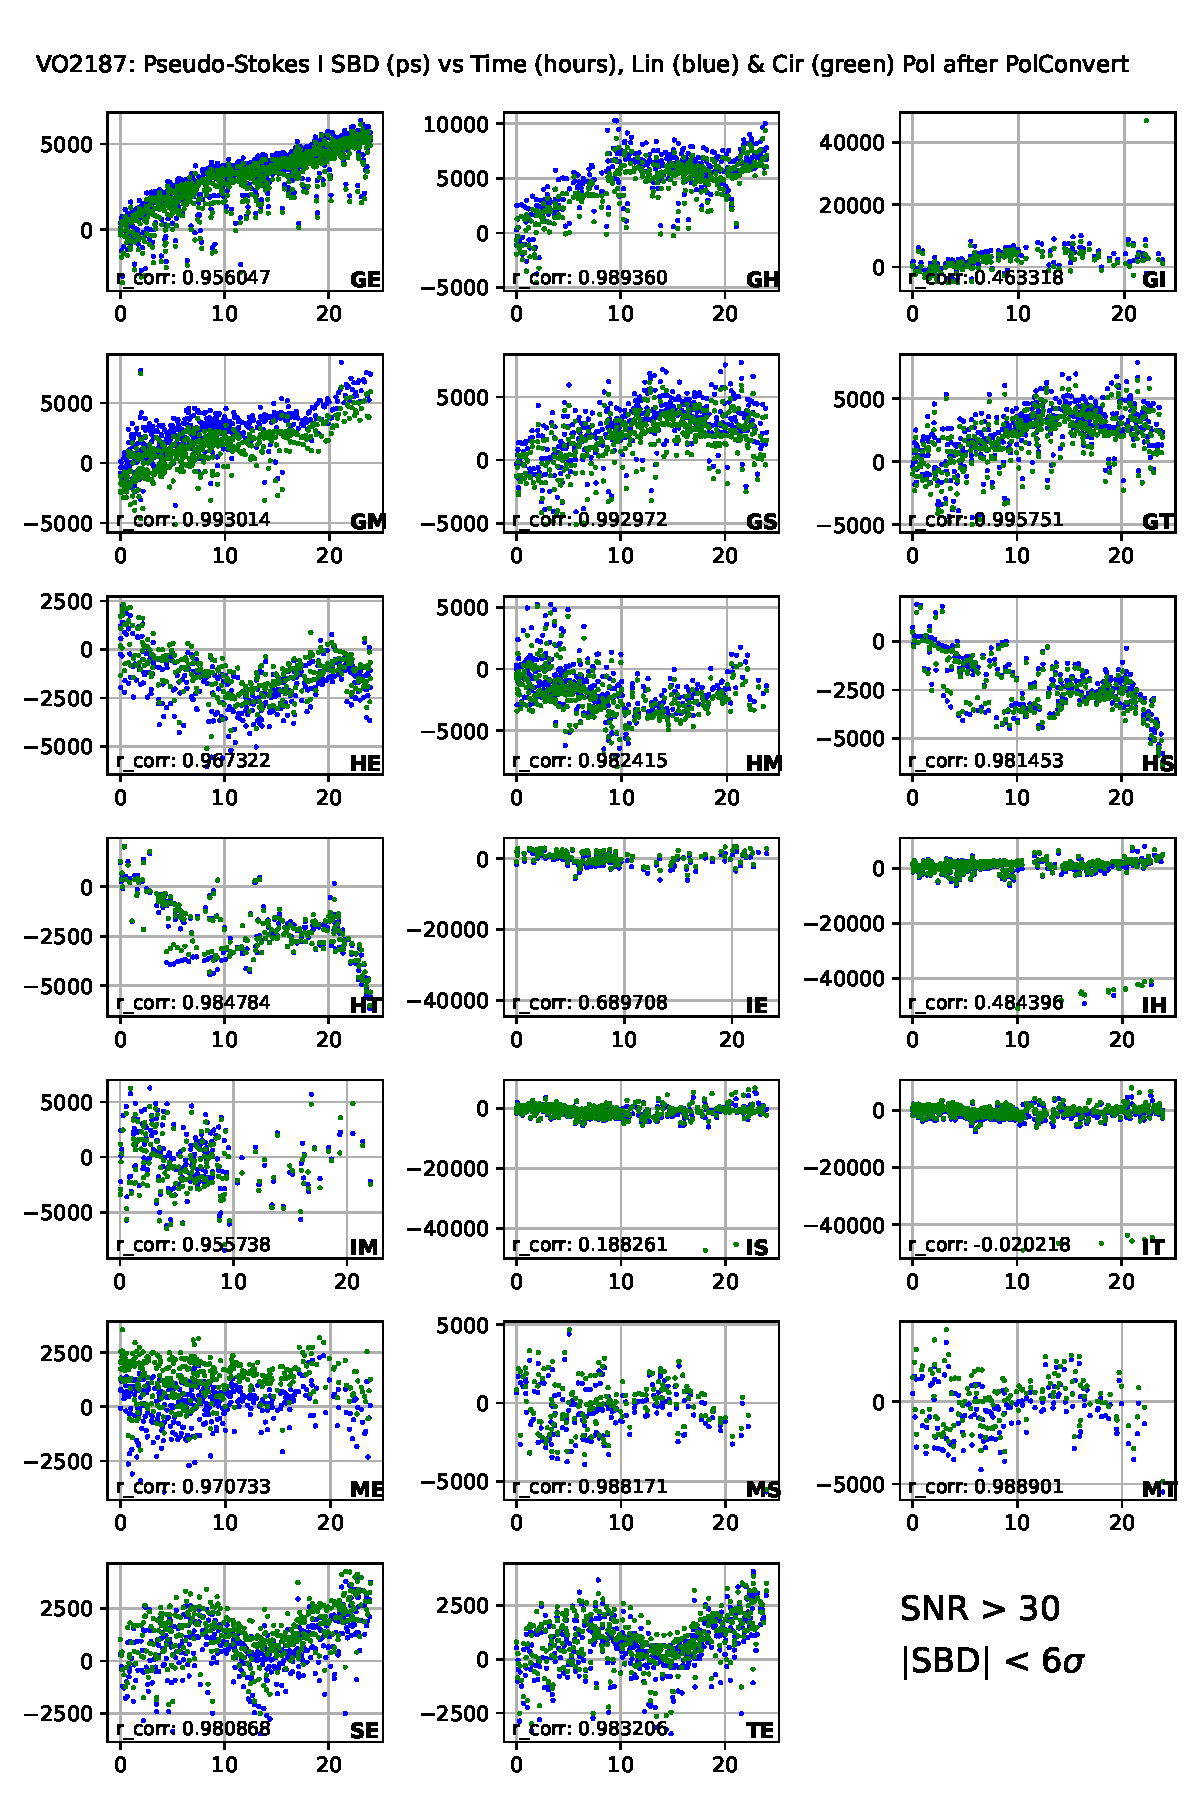
\includegraphics[width=33pc]{VO2187_SBD_Lin_I_and_Cir_I_SNR_floor_30.pdf}
  \caption{\small Evolution of Single-Band Delays (in picoseconds) during the experiment (time in minutes) for the pseudo-Stokes $\protect I$ parameter for every baseline. Each panel shows two curves: LinI, $\protect I$ from the original, linearly polarized data set and CirI, $\protect I$ from the circularly polarized data set obtained by applying PolConvert to the original data. Graphs have large biases. The coefficients of correlation r\_corr between Lin\_I and CirI for most of the baselines are close to unity. If it were not for the biases, the curves could be considered close to identical.}
  \label{sbd_lin_and_cir}
  \end{center}
\end{figure}


\begin{figure}[ht!]
  \begin{center}
  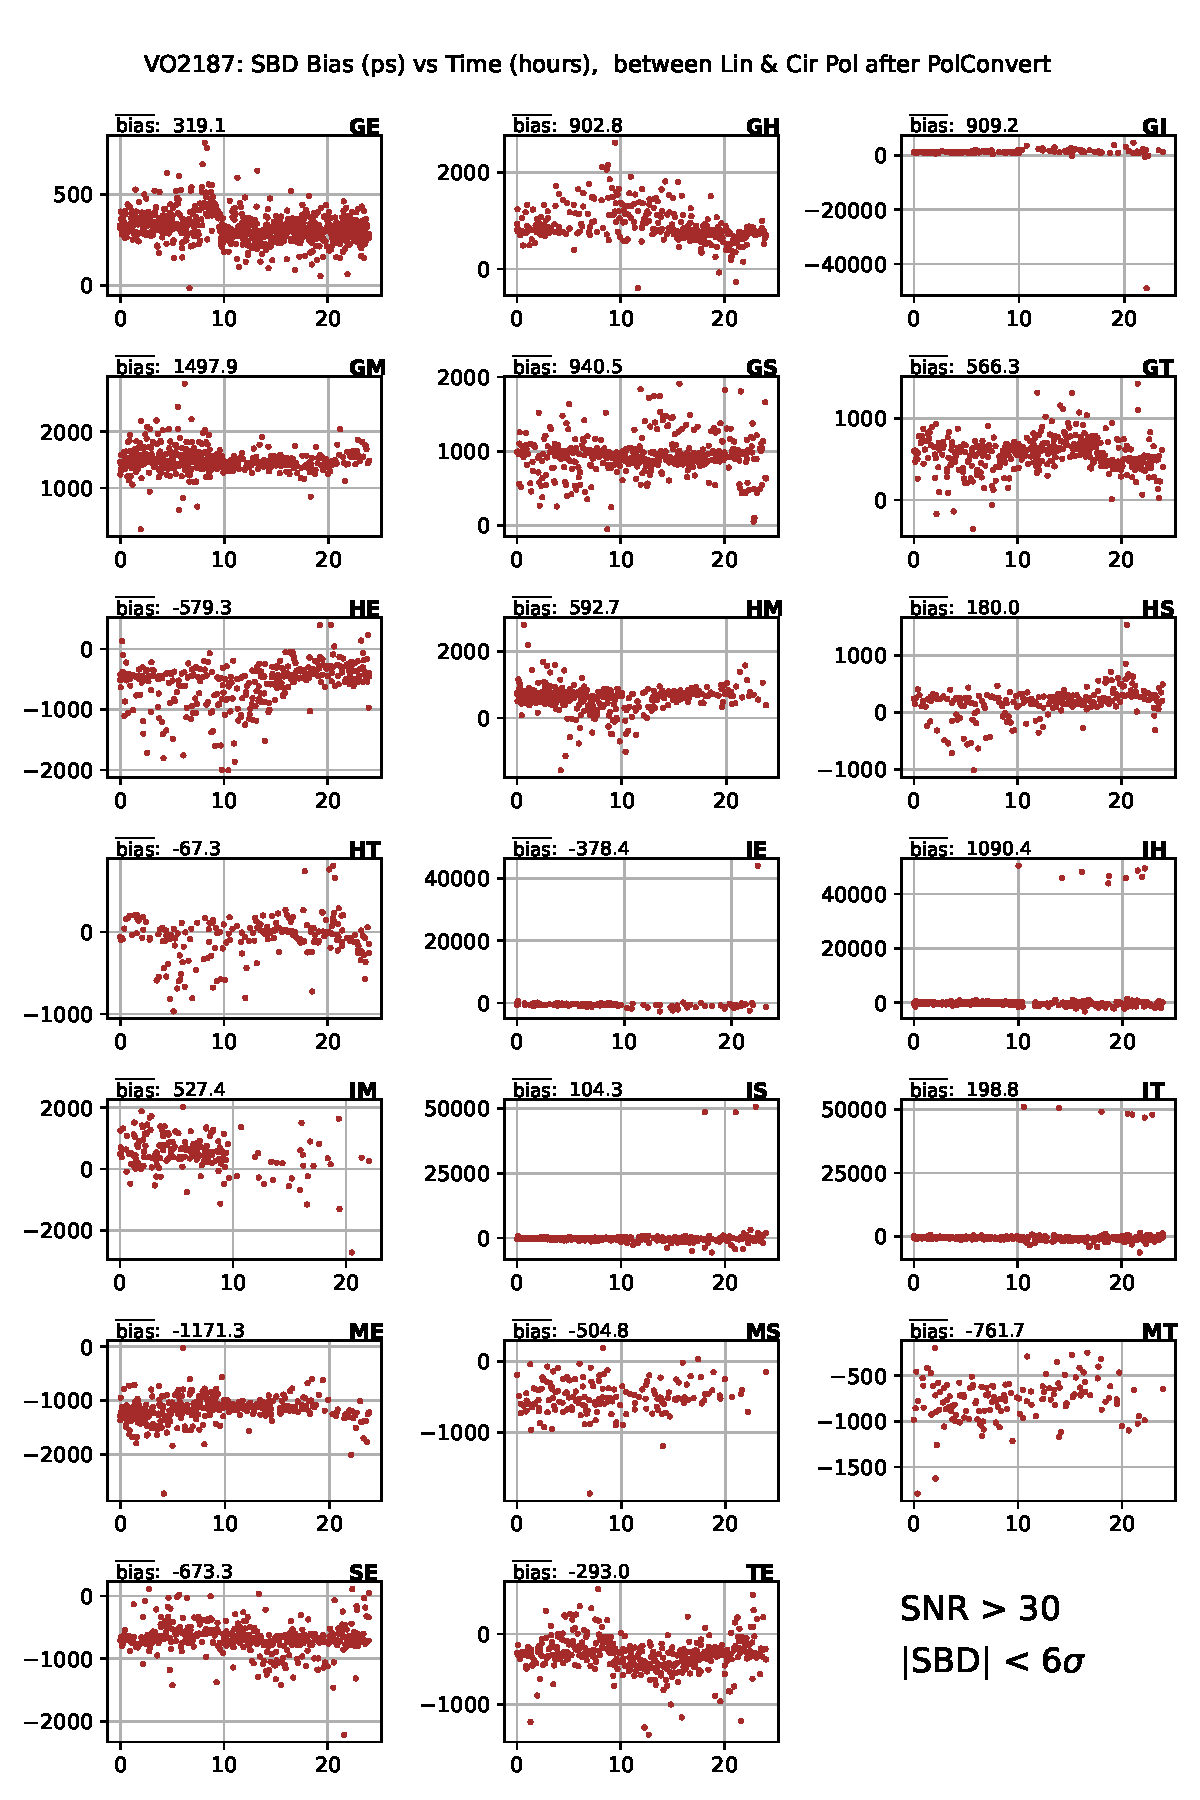
\includegraphics[width=33pc]{VO2187_SBD_bias_between_Lin_I_and_Cir_I_SNR_floor_30.pdf}
  \caption{\small Evolution of the bias between LinI and CirI Single-Band Delays (in picoseconds) during the experiment (time in minutes) for the pseudo-Stokes $\protect I$ parameter for every baseline. Each panel shows a curve of LinI - CirI, where LinI is $\protect I$ from the original, linearly polarized data set and CirI is $\protect I$ from the circularly polarized data set obtained by applying PolConvert to the original data. The means for each curve are given.}
  \label{sbd_lin_cir_bias}
  \end{center}
\end{figure}


\begin{figure}[ht!]
  \begin{center}
  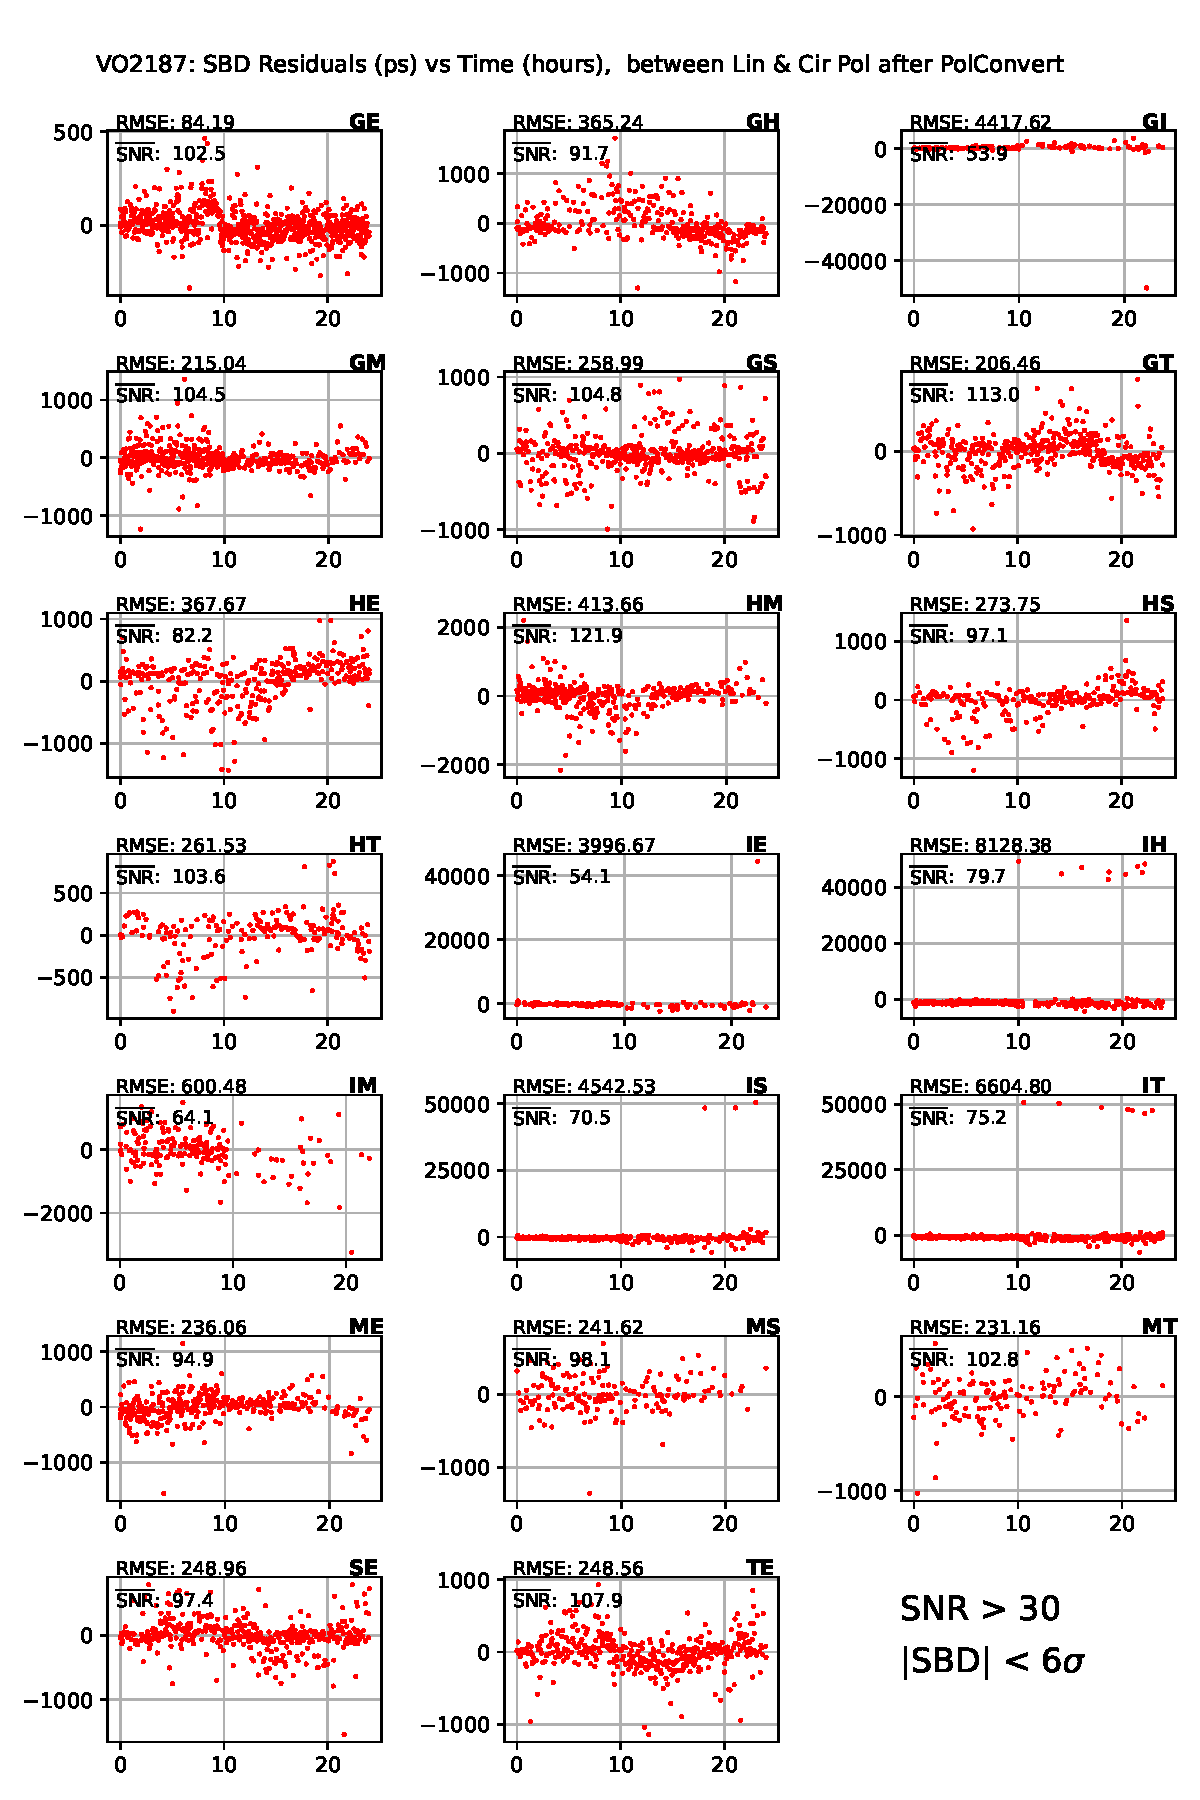
\includegraphics[width=33pc]{VO2187_SBD_Lin_I_minus_Cir_I_SNR_floor_30.pdf}
  \caption{\small Evolution of the residuals between unbiased LinI and CirI Single-Band Delays (in picoseconds) during the experiment (time in minutes) for the pseudo-Stokes $\protect I$ parameter for every baseline. Each panel shows a curve of LinI - CirI, both with subtracted means, where LinI is $\protect I$ from the original, linearly polarized data set and CirI is $\protect I$ from the circularly polarized data set obtained by applying PolConvert to the original data.  The Root Mean Square Error (RMSE) shows the standard deviation of the residuals.}
  \label{sbd_lin_minus_cir}
  \end{center}
\end{figure}


\begin{figure}[ht!]
  \begin{center}
  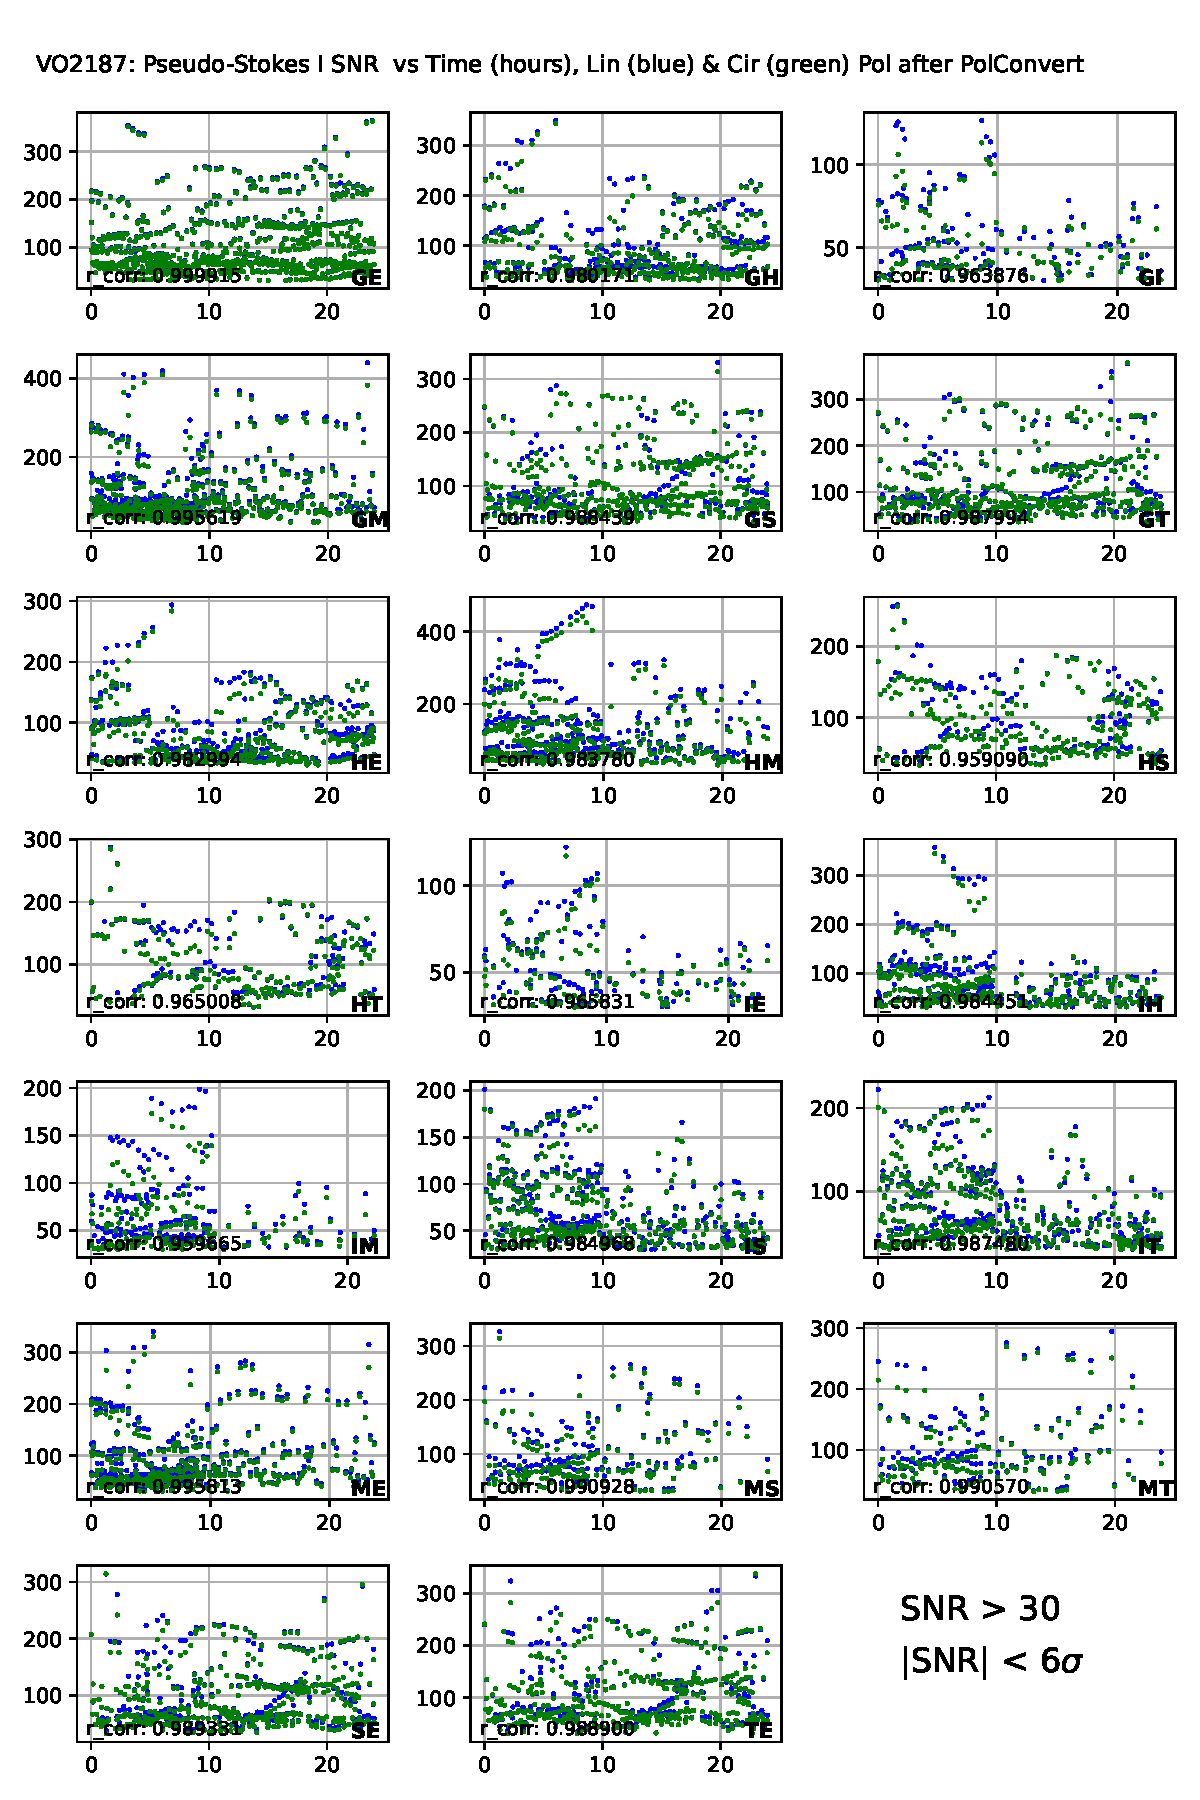
\includegraphics[width=33pc]{VO2187_SNR_Lin_I_and_Cir_I_SNR_floor_30.pdf}
  \caption{\small Evolution of Signal-to-Noise Ratios during the experiment (time in minutes) for the pseudo-Stokes $\protect I$ parameter for every baseline. Each panel shows two curves: LinI, $\protect I$ from the original, linearly polarized data set and CirI, $\protect I$ from the circularly polarized data set obtained by applying PolConvert to the original data. Graphs have large biases. }
  \label{snr_lin_and_cir}
  \end{center}
\end{figure}



\begin{figure}[ht!]
  \begin{center}
  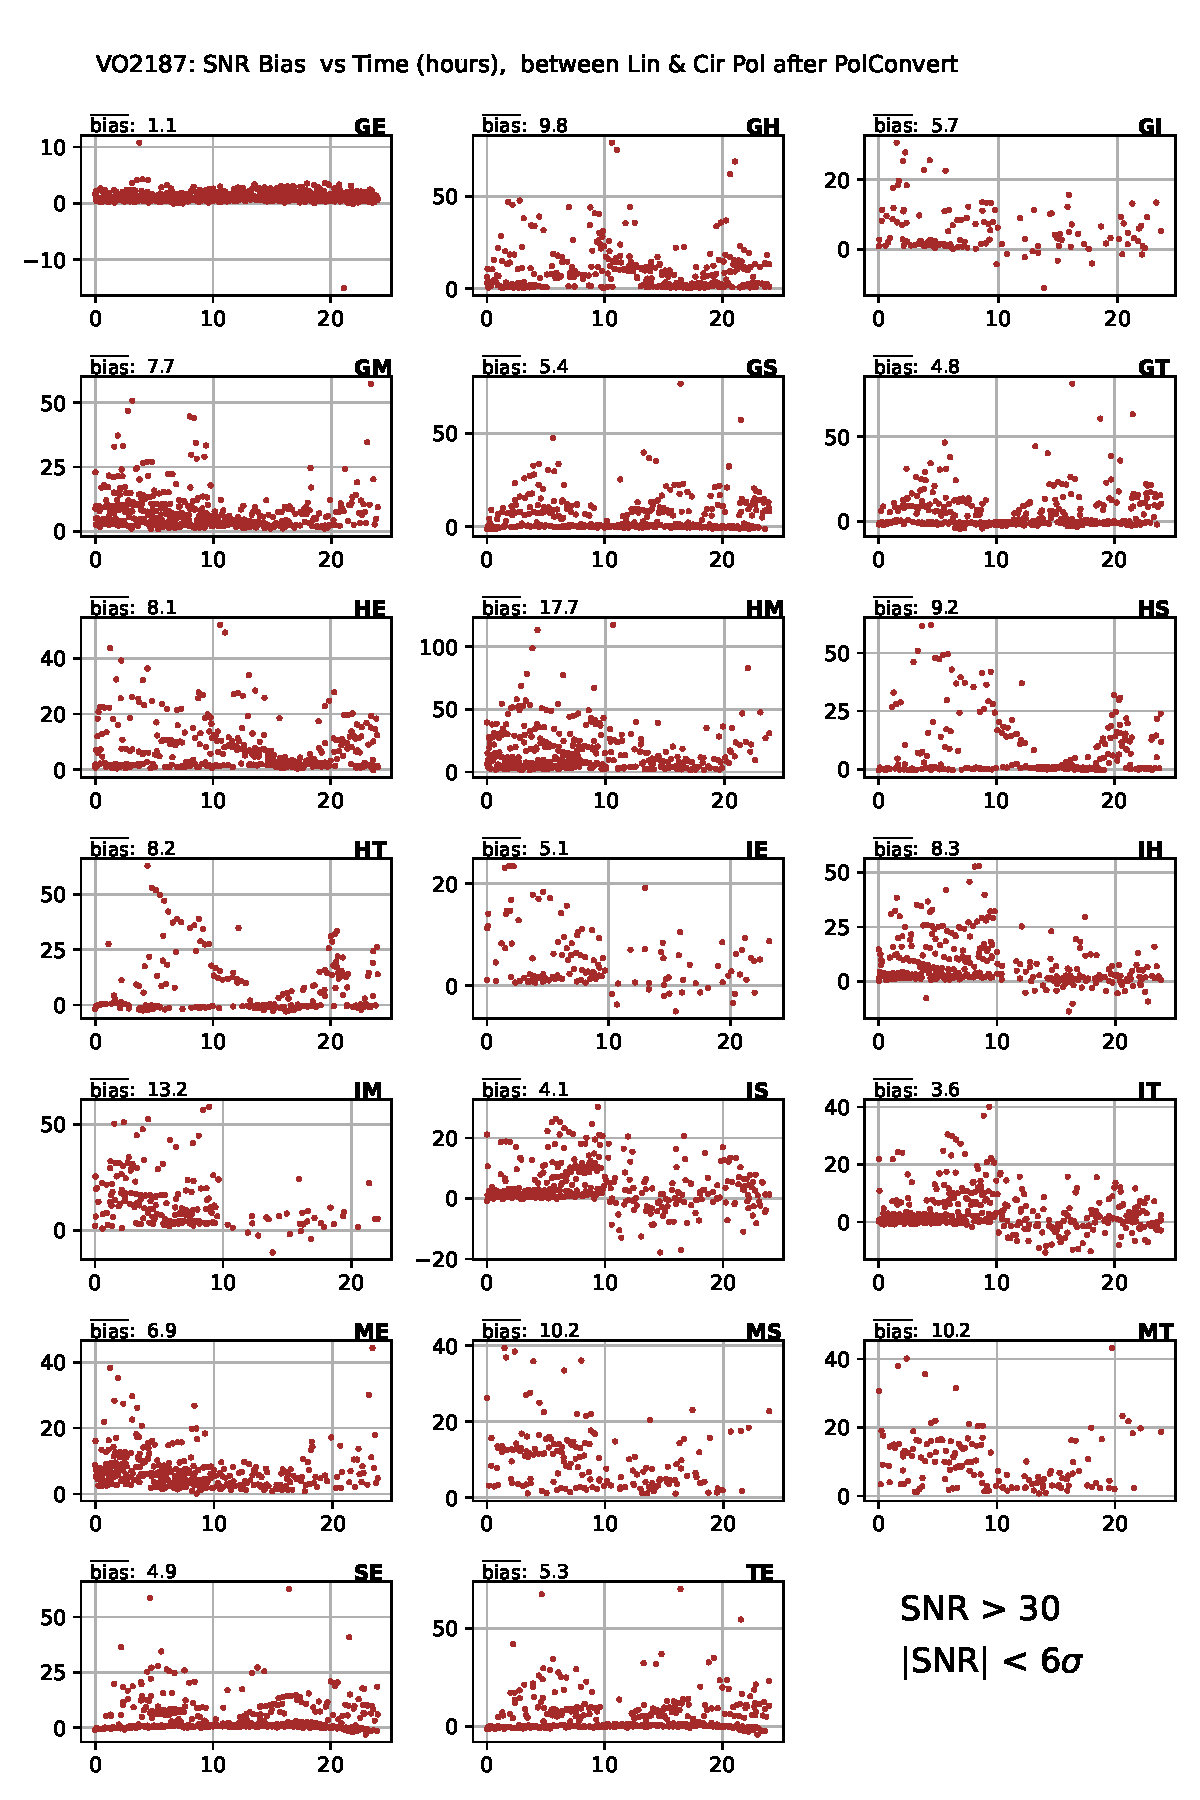
\includegraphics[width=33pc]{VO2187_SNR_bias_between_Lin_I_and_Cir_I_SNR_floor_30.pdf}
  \caption{\small Evolution of the bias between LinI and CirI Signal-to-Noise Ratios during the experiment (time in minutes) for the pseudo-Stokes $\protect I$ parameter for every baseline. Each panel shows a curve of LinI - CirI, where LinI is $\protect I$ from the original, linearly polarized data set and CirI is $\protect I$ from the circularly polarized data set obtained by applying PolConvert to the original data. The means for each curve are given.}
  \label{snr_lin_cir_bias}
  \end{center}
\end{figure}


\begin{figure}[ht!]
  \begin{center}
  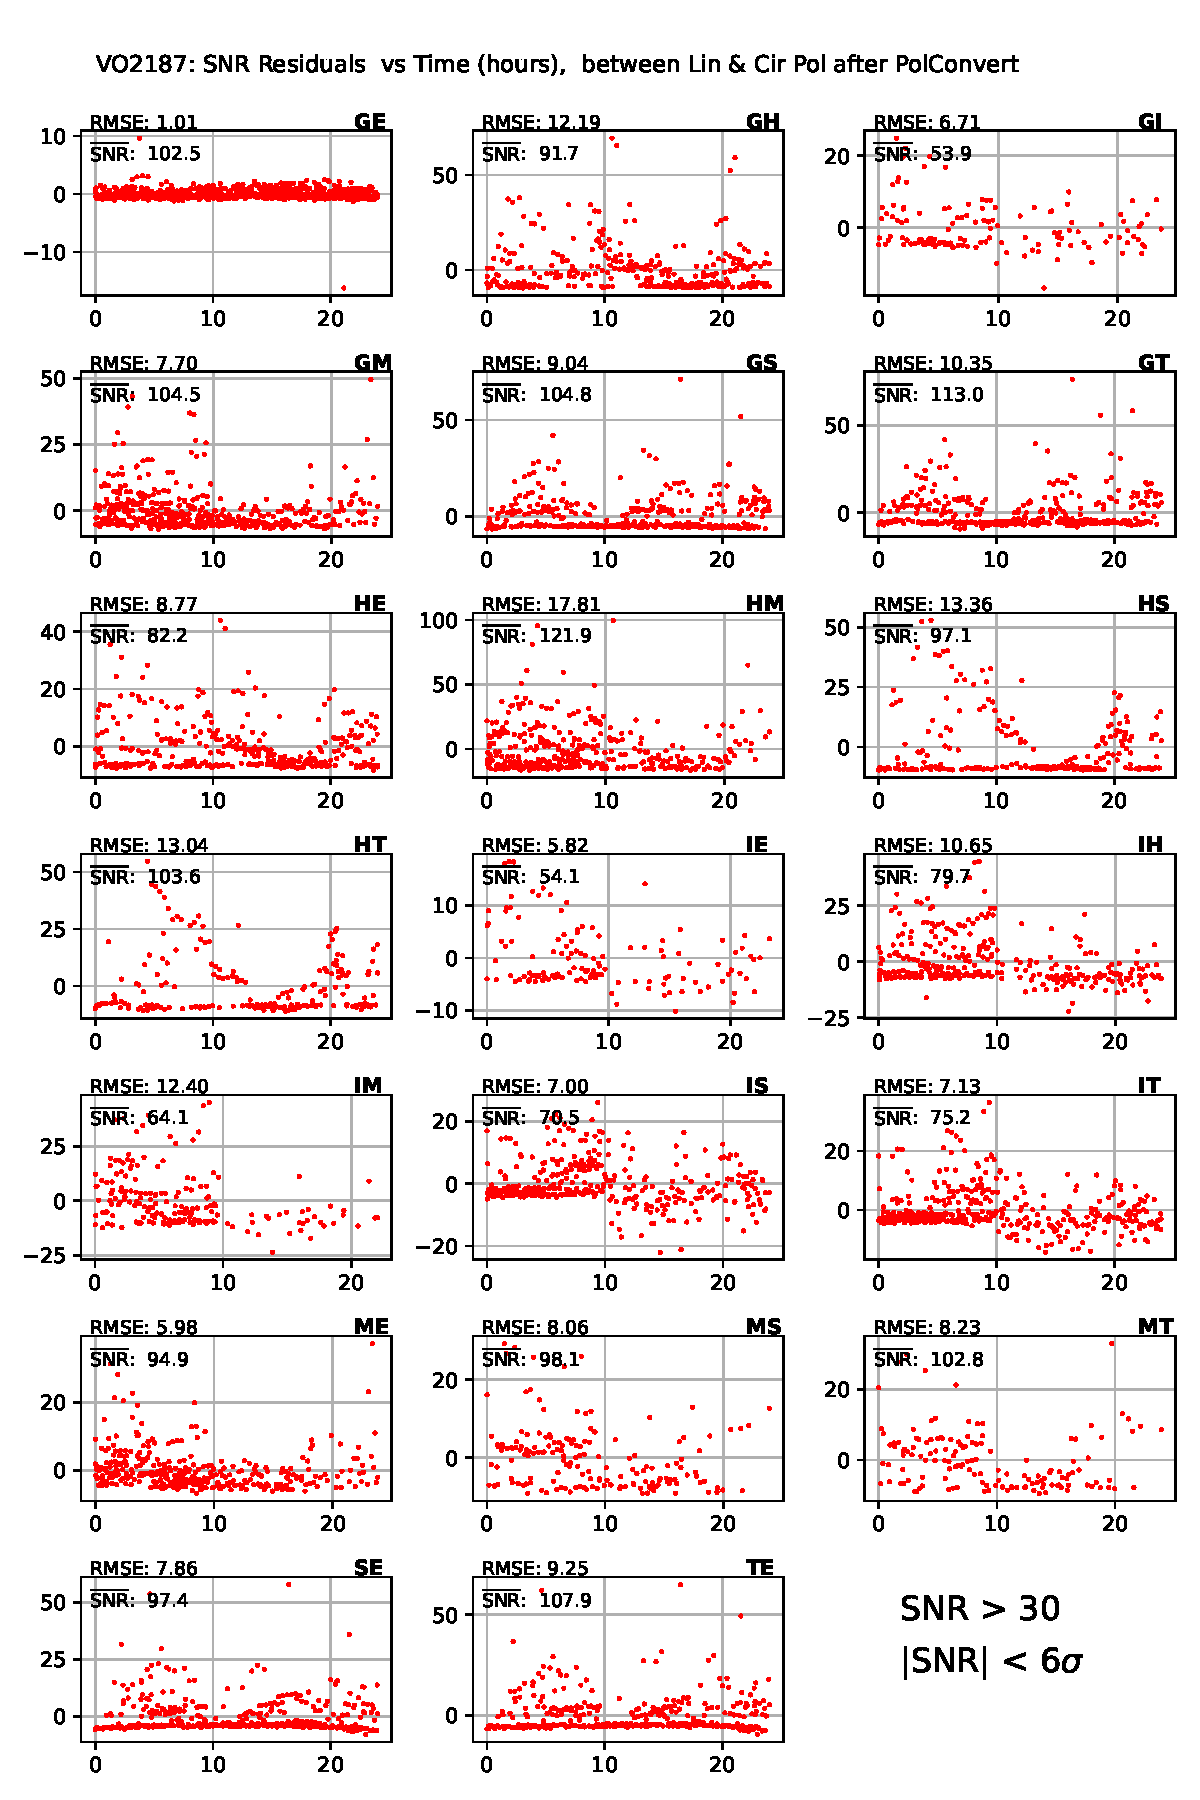
\includegraphics[width=33pc]{VO2187_SNR_Lin_I_minus_Cir_I_SNR_floor_30.pdf}
  \caption{\small  Evolution of the residuals between unbiased LinI and CirI Signal-to-Noise Ratios during the experiment (time in minutes) for the pseudo-Stokes $\protect I$ parameter for every baseline. Each panel shows a curve of LinI - CirI, both with subtracted means, where LinI is $\protect I$ from the original, linearly polarized data set and CirI is $\protect I$ from the circularly polarized data set obtained by applying PolConvert to the original data. The time-averaged SNRs are provided. The Root Mean Square Error (RMSE) shows the standard deviation of the residuals. The coefficients of correlation r\_corr between LinI and CirI are very close to unity.}
  \label{snr_lin_minus_cir}
  \end{center}
\end{figure}





\begin{figure}[ht!]
  \begin{center}
  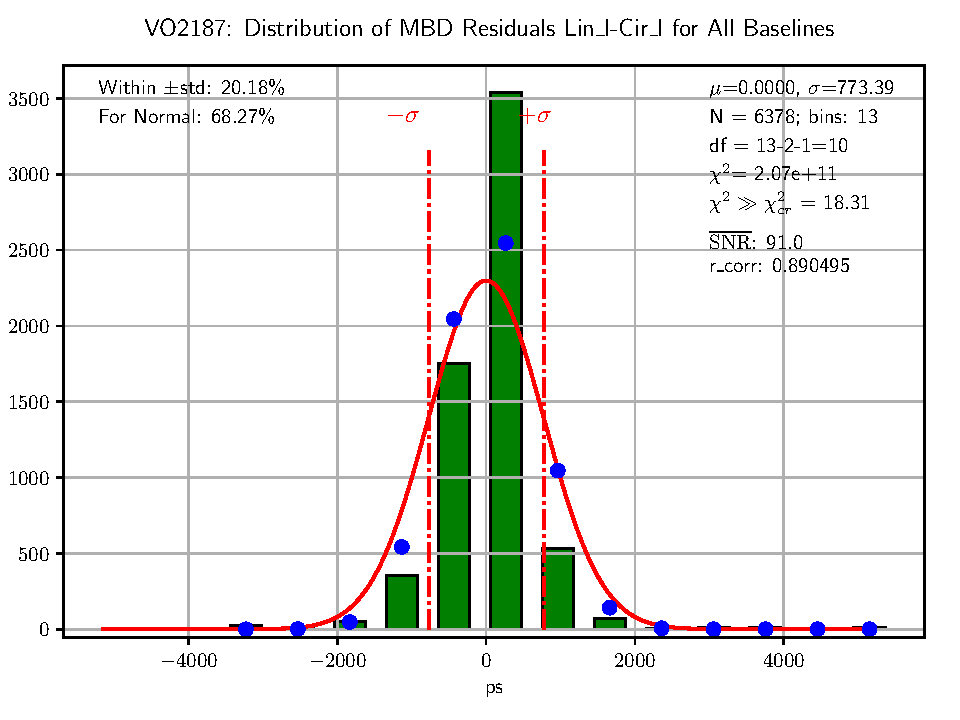
\includegraphics[width=25pc]{VO2187_Distr_MBD_Lin_I-Cir_I_Diff.pdf}
  \caption{\small Histogram of the Multi-Band Delay residuals (see Eq.~\eqref{resid}) for all of the baselines. N is the total number of residuals spread over 21 bin. For the Pearson's $\chi^2$ test, the left-tail and right-tail bins with sparse data (less than 5 counts in each) were grouped to make only $N_b=8$ bins. The number of degrees of freedom df is 5 (i.e. $N_b-3$). With this df, the critical value, $\chi^2_{cr}$ is 11.07. The $\chi^2$ observed, 183.48, greatly exceeds $\chi^2_{cr}$, so the test fails. However, the proportion of residuals within $\pm\sigma$, 83.8\%, is much better than 68.27\% of a normal distribution.}
  \label{dmbd_distr}
  \end{center}
\end{figure}


\begin{figure}[ht!]
  \begin{center}
  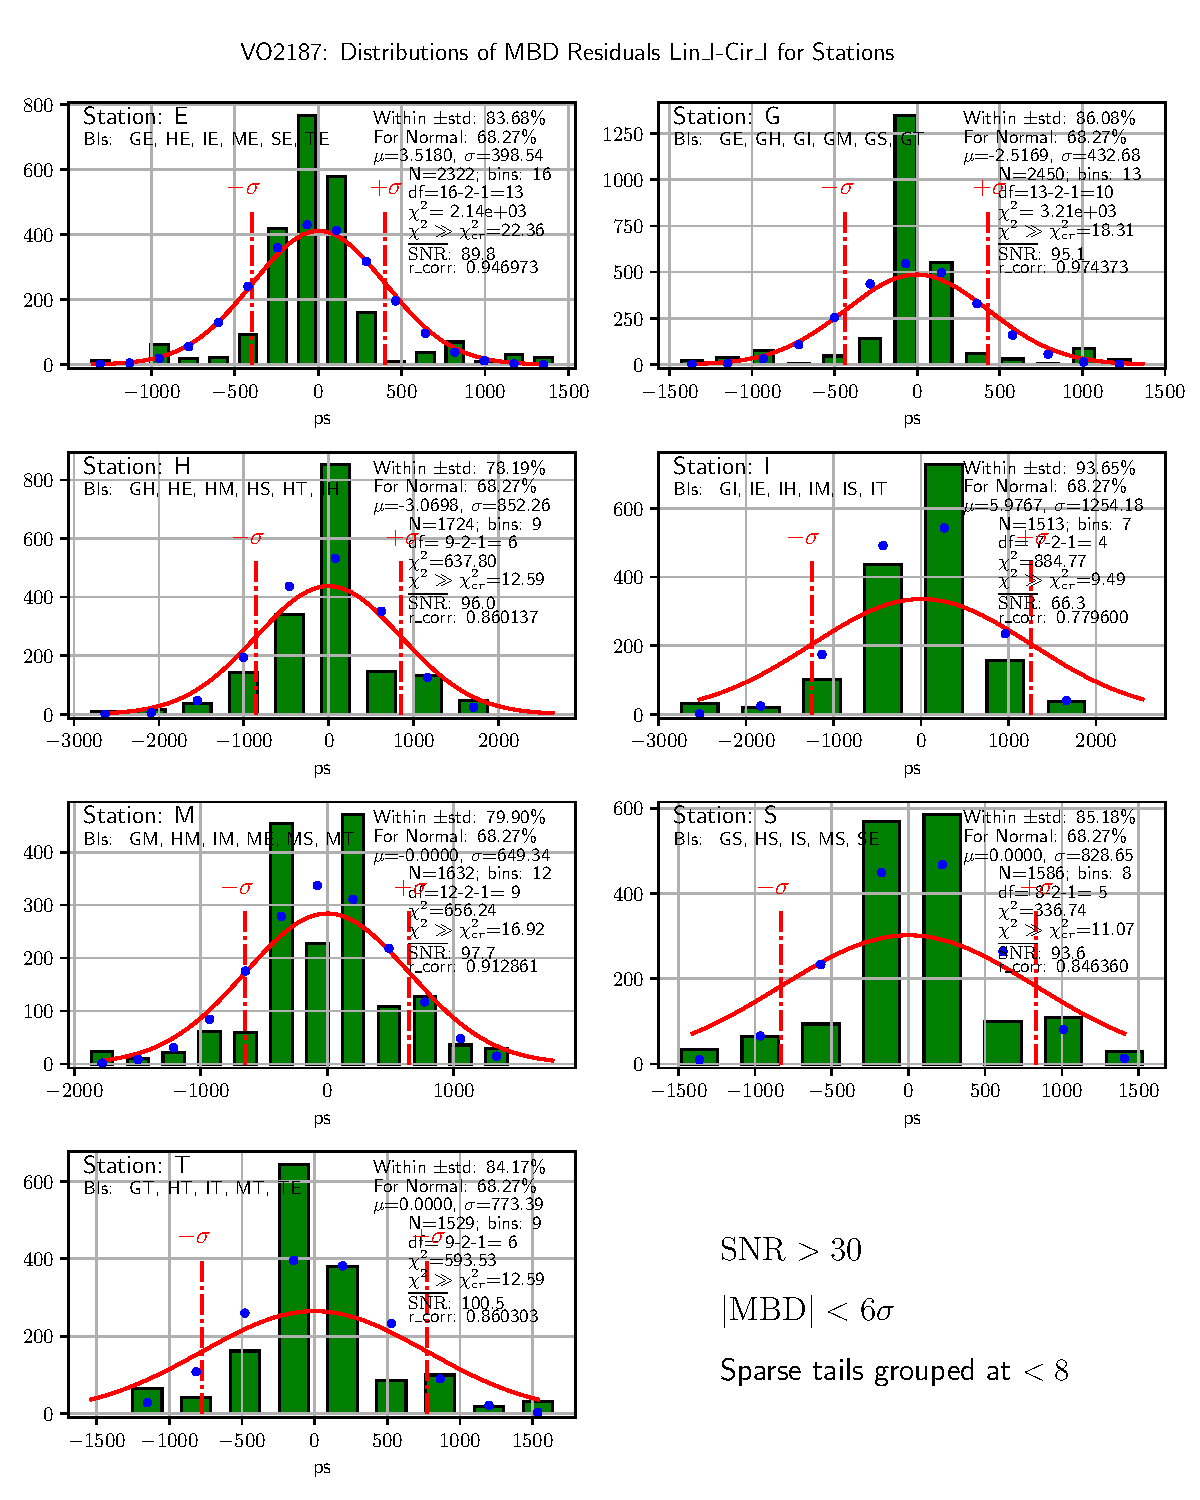
\includegraphics[width=33pc]{VO2187_Distr_MBD_Lin_I-Cir_I_Diff_Stations.pdf}
  \caption{\small Histograms of the Multi-Band Delay residuals (see Eq.~\eqref{resid}) for the groups of baselines including an individual station. N is the total number of residuals spread over 21 bin. For the Pearson's $\chi^2$ test, the left-tail and right-tail bins with sparse data (less than 5 counts in each) were grouped to make smaller number of bins $N_b$. The number of degrees of freedom df is $N_b-3$. With these df, the critical values $\chi^2_{cr}$ are calculated. For all the distributions, the $\chi^2$ observed exceed $\chi^2_{cr}$, so the tests fail. However, the proportions of residuals within $\pm\sigma$ are much better than 68.27\% of a normal distribution.}
  \label{dmbd_distr_st}
  \end{center}
\end{figure}


\begin{figure}[ht!]
  \begin{center}
  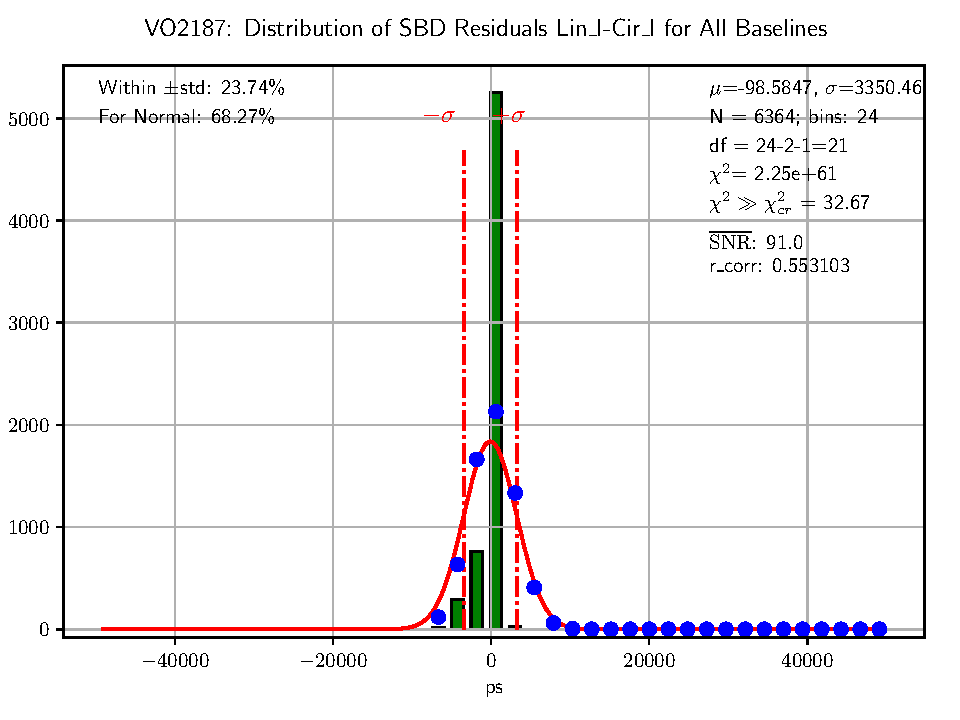
\includegraphics[width=25pc]{VO2187_Distr_SBD_Lin_I-Cir_I_Diff.pdf}
  \caption{\small Histogram of the Single-Band Delay residuals (see Eq.~\eqref{resid}) for all of the baselines. N is the total number of residuals spread over 21 bin. For the Pearson's $\chi^2$ test, the left-tail and right-tail bins with sparse data (less than 5 counts in each) were grouped to make only $N_b=9$ bins. The number of degrees of freedom df is 6 (i.e. $N_b-3$). With this df, the critical value, $\chi^2_{cr}$ is 12.59. The $\chi^2$ observed, 44.99, significantly exceeds $\chi^2_{cr}$, so the test fails. However, the proportion of residuals within $\pm\sigma$, 77.19\%, is much better than 68.27\% of a normal distribution.}
  \label{dsbd_distr}
  \end{center}
\end{figure}


\begin{figure}[ht!]
  \begin{center}
  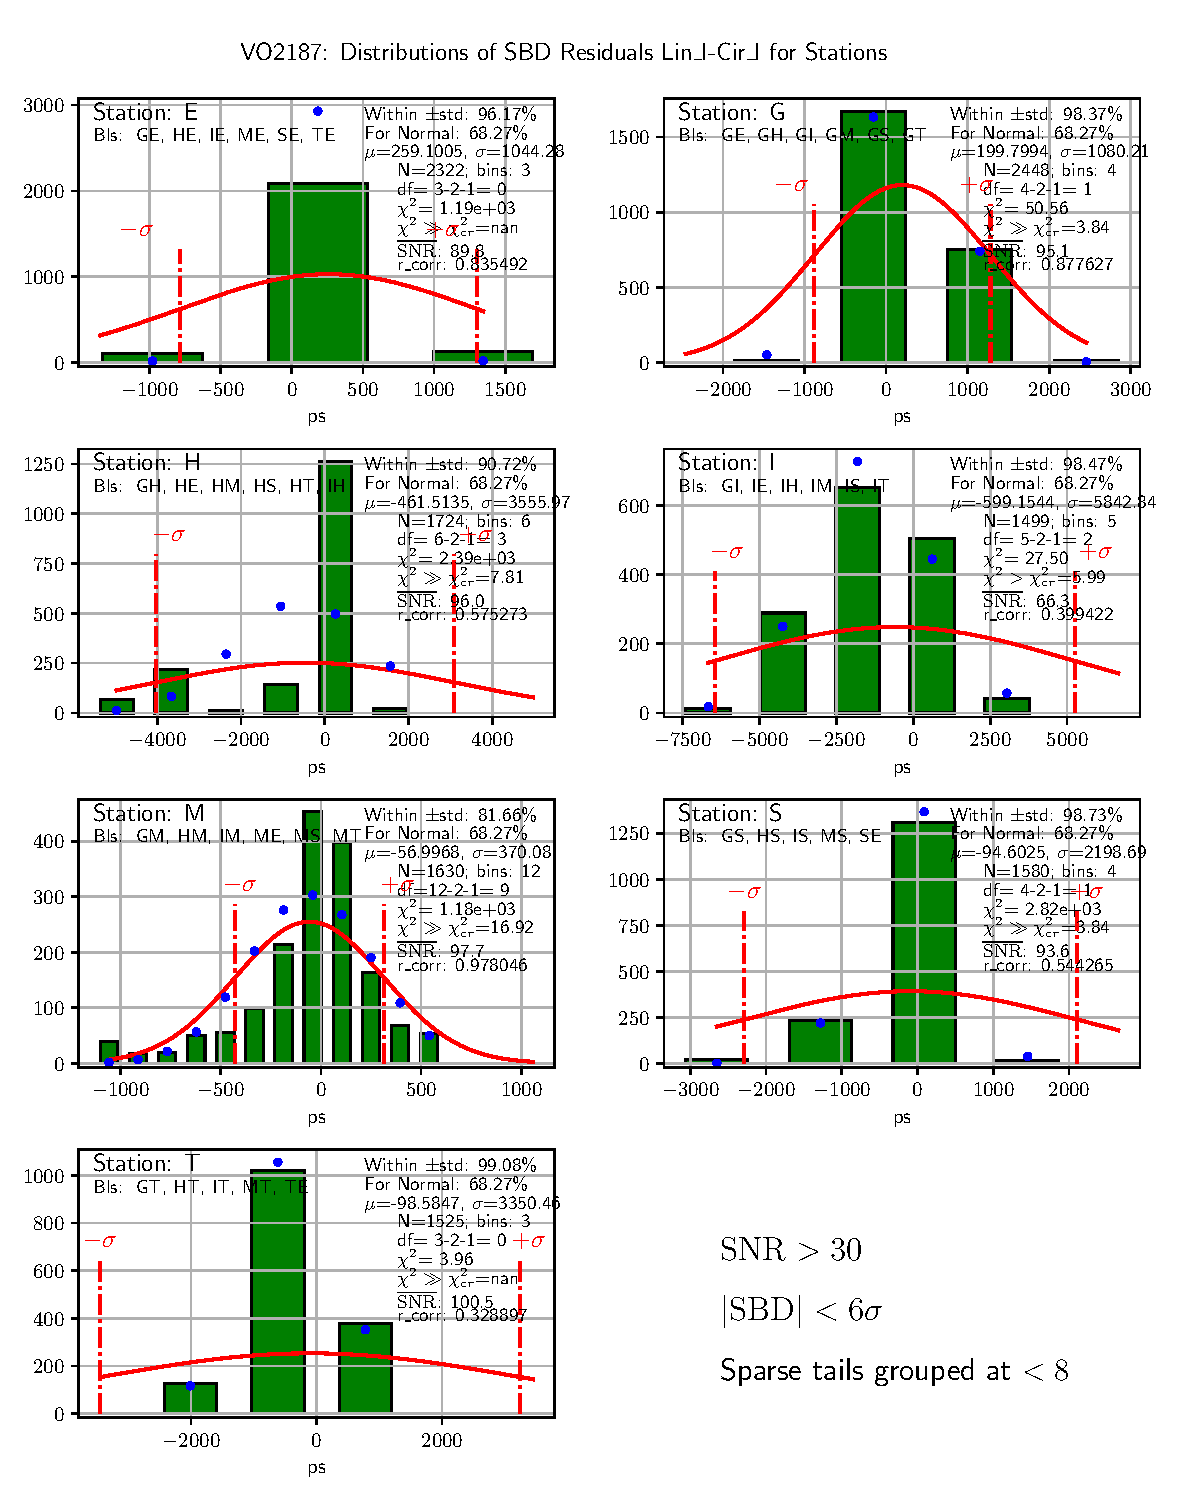
\includegraphics[width=33pc]{VO2187_Distr_SBD_Lin_I-Cir_I_Diff_Stations.pdf}
  \caption{\small Histograms of the Single-Band Delay residuals (see Eq.~\eqref{resid}) for the groups of baselines including an individual station. N is the total number of residuals spread over 21 bin. For the Pearson's $\chi^2$ test, the left-tail and right-tail bins with sparse data (less than 5 counts in each) were grouped to make smaller number of bins $N_b$. The number of degrees of freedom df is $N_b-3$. With these df, the critical values $\chi^2_{cr}$ are calculated. For most of the distributions (except those including stations E and V), the $\chi^2$ observed exceed $\chi^2_{cr}$, so the tests fail. Stations E and V have normally distributed residuals with 95\% confidence. However, for all of the stations, the proportions of residuals within $\pm\sigma$ are better than 68.27\% of a normal distribution.}
  \label{dsbd_distr_st}
  \end{center}
\end{figure}


\begin{figure}[ht!]
  \begin{center}
  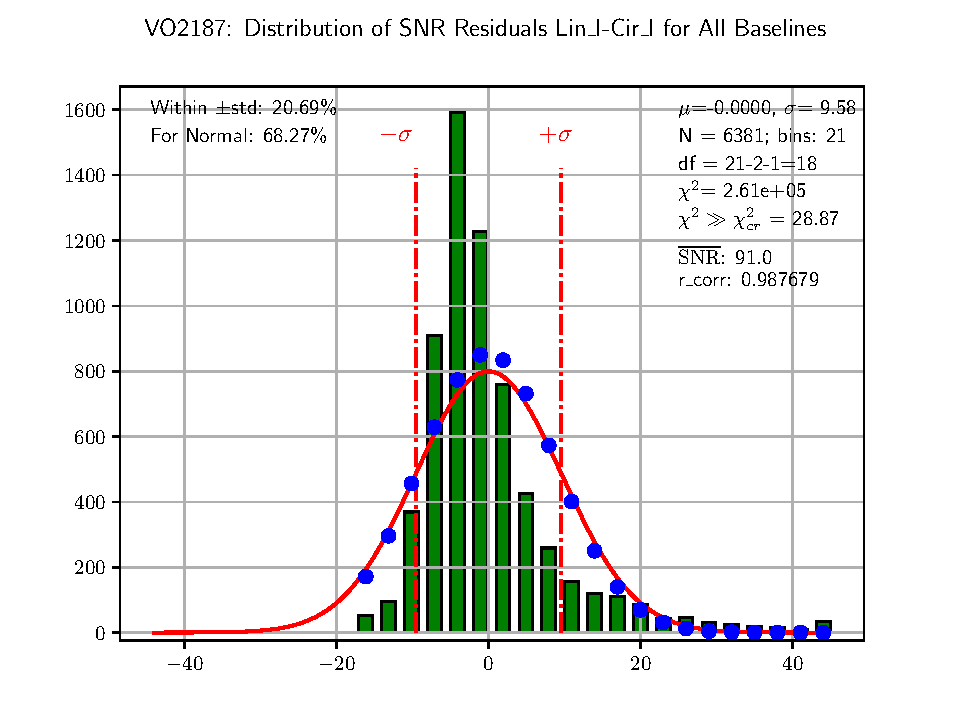
\includegraphics[width=25pc]{VO2187_Distr_SNR_Lin_I-Cir_I_Diff.pdf}
  \caption{\small  Histogram of the Signal-to-Noise Ratio residuals (see Eq.~\eqref{resid}) for all of the baselines. N is the total number of residuals spread over 21 bin. For the Pearson's $\chi^2$ test, the left-tail and right-tail bins with sparse data (less than 5 counts in each) were grouped to make only $N_b=11$ bins. The number of degrees of freedom df is 8 (i.e. $N_b-3$). With this df, the critical value, $\chi^2_{cr}$ is 15.51. The $\chi^2$ observed, 130.72, greatly exceeds $\chi^2_{cr}$, so the test fails. However, the proportion of residuals within $\pm\sigma$, 82.94\%, is much better than 68.27\% of a normal distribution.}
  \label{dsnr_distr}
  \end{center}
\end{figure}



\begin{figure}[ht!]
  \begin{center}
  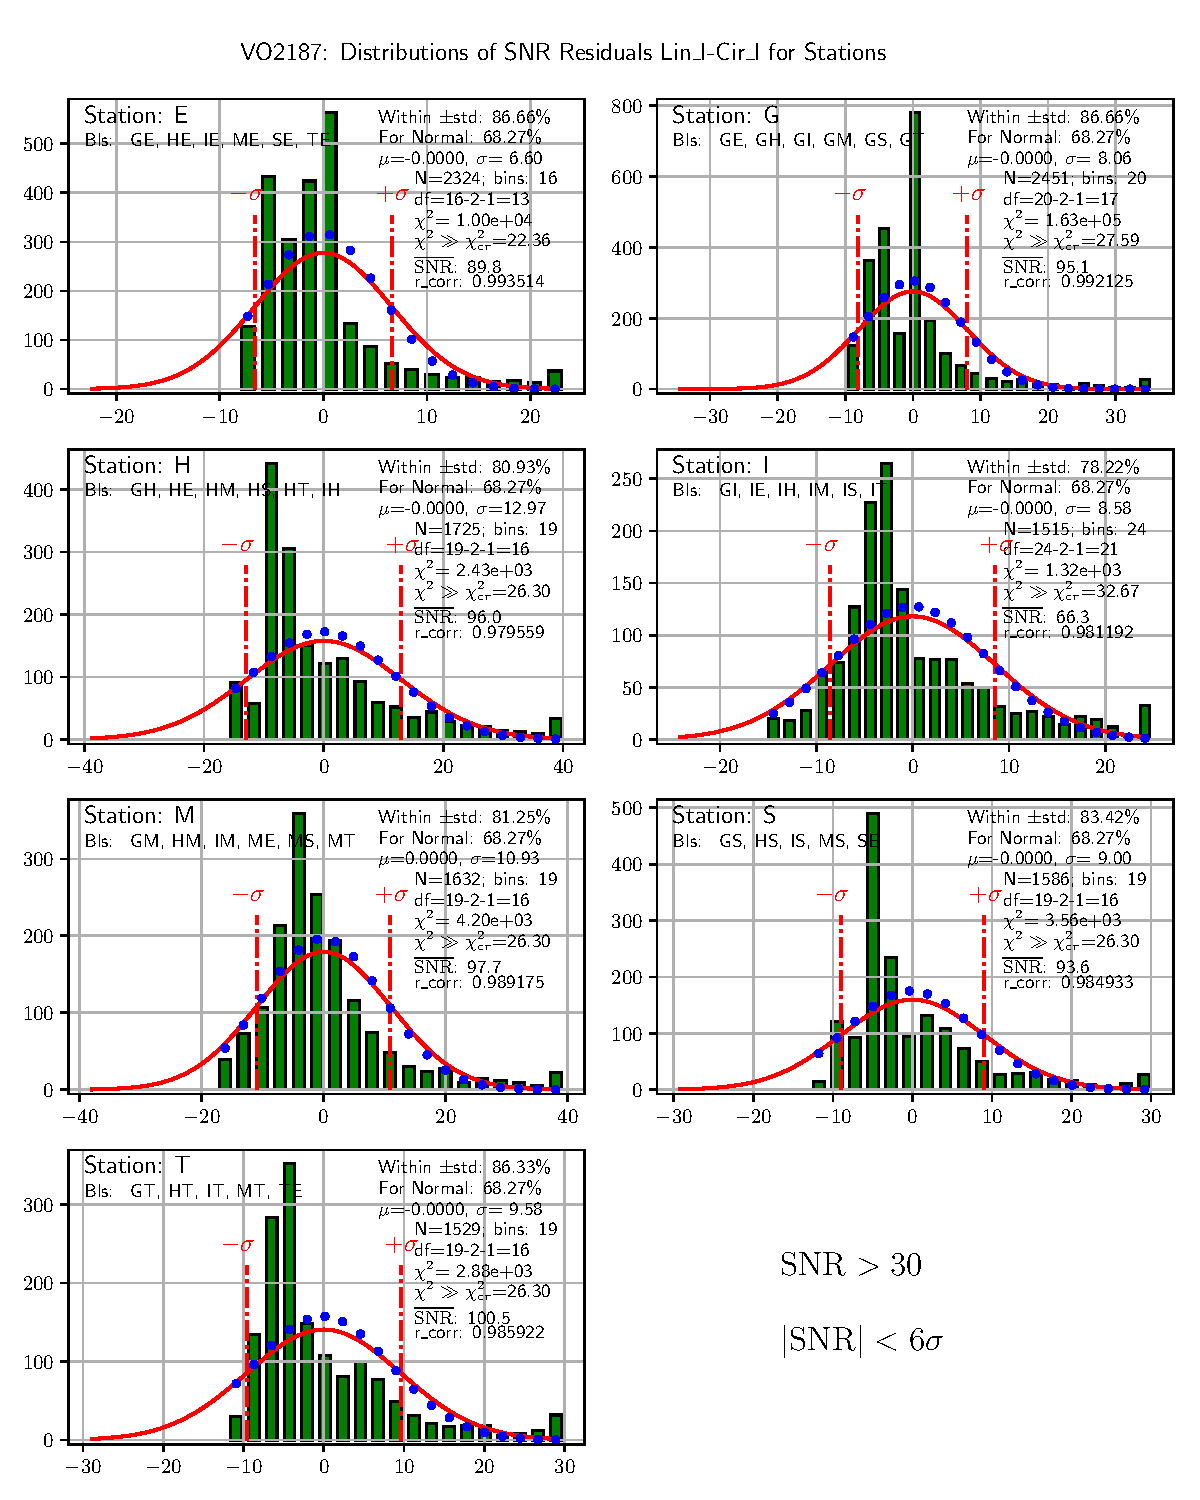
\includegraphics[width=33pc]{VO2187_Distr_SNR_Lin_I-Cir_I_Diff_Stations.pdf}
  \caption{\small Histograms of the Signal-to-Noise Ratio residuals (see Eq.~\eqref{resid}) for the groups of baselines including an individual station. N is the total number of residuals spread over 21 bin. For the Pearson's $\chi^2$ test, the left-tail and right-tail bins with sparse data (less than 5 counts in each) were grouped to make smaller number of bins $N_b$. The number of degrees of freedom df is $N_b-3$. With these df, the critical values $\chi^2_{cr}$ are calculated. For all the distributions, the $\chi^2$ observed exceed $\chi^2_{cr}$, so the tests fail. However, the proportions of residuals within $\pm\sigma$  (except station M with its 64.81\%) are much better than 68.27\% of a normal distribution. }
  \label{dsnr_distr_st}
  \end{center}
\end{figure}




\end{document}



